\documentclass[UTF8]{ctexart}
\usepackage{graphicx}
\usepackage{authblk}
\usepackage{subfigure}
\usepackage[headheight=12.64723pt]{geometry}
\geometry{a4paper, centering, scale = 0.8}
\usepackage[format = hang, font = small, textfont = it]{caption}
\usepackage{fancyhdr}
\usepackage{caption}

\usepackage{amsmath}
\usepackage{amsfonts}
\usepackage{epstopdf}
\usepackage{fontspec}
\usepackage{color}
\usepackage{xcolor}
\setmonofont{Consolas}

\usepackage{pifont}
\usepackage{extarrows}
\usepackage{harpoon}
\usepackage{bm}
\usepackage{esint}

\usepackage{listings}
\usepackage{enumerate}

\usepackage{makecell}
\usepackage{appendix}
\usepackage{hyperref}
\hypersetup{
    colorlinks=true,
    linkcolor=blue,
    filecolor=blue,
    urlcolor=blue,
    citecolor=cyan,
}
\usepackage{media9}
\usepackage[numbers,super]{natbib} % it seems that it needs bibliographystyle settings
\usepackage{bookmark}

\pagestyle{fancy}
\lhead{}
\chead{\leftmark}
\rhead{\rightmark}
\lfoot{}
\cfoot{- \thepage\ -}
% \rfoot{范皓年}
\rfoot{}
\renewcommand{\headrulewidth}{0.4pt}
\renewcommand{\footrulewidth}{0.4pt}

\lstset{
    numbers=left,
    columns=fixed,
    rulesepcolor=\color{red!20!green!20!blue!20},
    basicstyle=\ttfamily,                                      % 在左侧显示行号
    numberstyle=\tiny\color{gray},                       % 设定行号格式
    frame=shadowbox,                                          % 不显示背景边框
    backgroundcolor=\color[RGB]{245,245,244},            % 设定背景颜色
    keywordstyle=\color[RGB]{40,40,255},                 % 设定关键字颜色
    numberstyle=\footnotesize\color{darkgray},
    commentstyle=\it\color[RGB]{0,96,96},                % 设置代码注释的格式
    stringstyle=\rmfamily\slshape\color[RGB]{128,0,0},   % 设置字符串格式
    showstringspaces=false,                              % 不显示字符串中的空格
    language=python                                      % 设置语言
}
\bibliographystyle{plain}

    \title{\heiti {科技交流与写作课程论文} \\ \Huge 最小生成树算法的对比分析\\ \huge Kruskal, Prim及其堆优化}
    \author{\kaishu 袁世平\footnote{1700012899,计算机科学与技术系},范皓年\footnote{1900012739, 电子信息工程系}}
    \date{\today}

%%%%%%%%%%%%%%%%%%%%%%%%%%%%%%%%%%%%%%%%%%%%%%%%%%%%%%%%%%%%%%%%%%%
\begin{document}
\maketitle

\tableofcontents
\newpage
\section{引言}
网络无处不在,对于已有的稍见规模的社会系统,和现在逐渐发展蓬勃的互联网系统,都存在连接和组织的问题。为了联系一个网络系统当中的各个节点,我们需要构建连通图。

在实际生活中,由于工程难度和用户协调等等问题,成本相差极大,构建不同方案的连通图将会有较大的财力和时间成本的差异,所以这个问题有着重大的研究价值。

对于n个节点组成的图,所有可能的连接共\(\frac{n(n-1)}{2}\)条,为构建一个边权最低的连通图,我们需要从中选取\(n-1\)条权值最低的边,求解一个连通图的最小连通分支的问题就是最小生成树问题。

已有的比较成熟的最小生成树算法有“Prim算法”,“Kruskal算法”\cite{RN4},以及时常为了减小Prim的遍历的时间开销而进行优化的“带堆优化的Prim算法”。但由于带有堆优化的Prim算法相对于其他两种算法优势过于显著(耗时低约3个量级),所以主要研究朴素Prim和Kruskal两种算法,对图中各边进行等权、排列权、随机权值的实验验证,探讨常见的MST算法在应用中的优劣。


\section{理论分析}\label{sec:theo}
\subsection{Prim算法} 

Prim算法\cite{RN3}是一种基于节点查找的最小生成树算法,基本思想是从一个结点开始,不断加点(而不是 Kruskal 算法的加边)。具体来说,未加入结点中距离已加入结点最小的结点,并用这个结点的邻边更新与其他未加入结点的距离。

\begin{figure}[htbp]
    \centering
    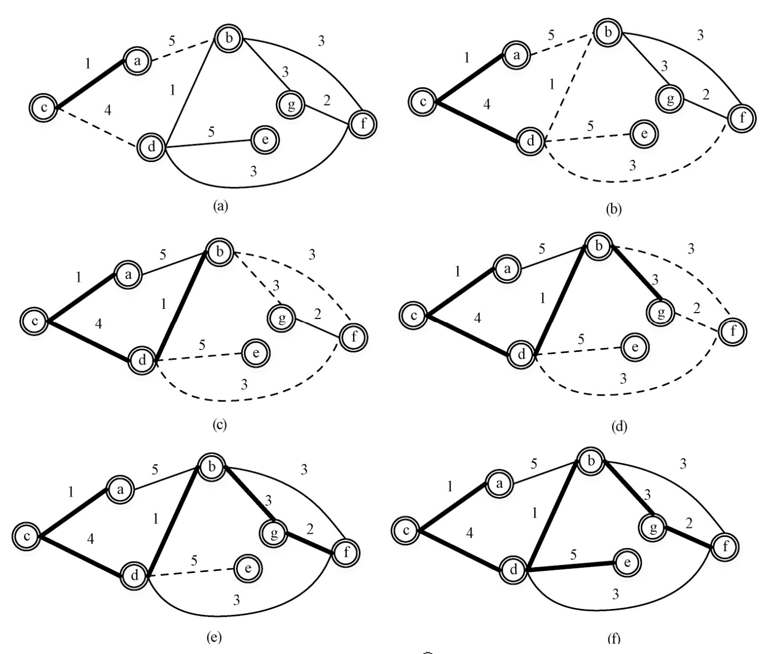
\includegraphics[width=0.7\textwidth]{assets/prim.png}
    \caption{Prim算法的过程示例}
    \label{fig:prim}
\end{figure}\cite{贺军忠2020kruskal}
\begin{figure}[htbp]
    \centering
    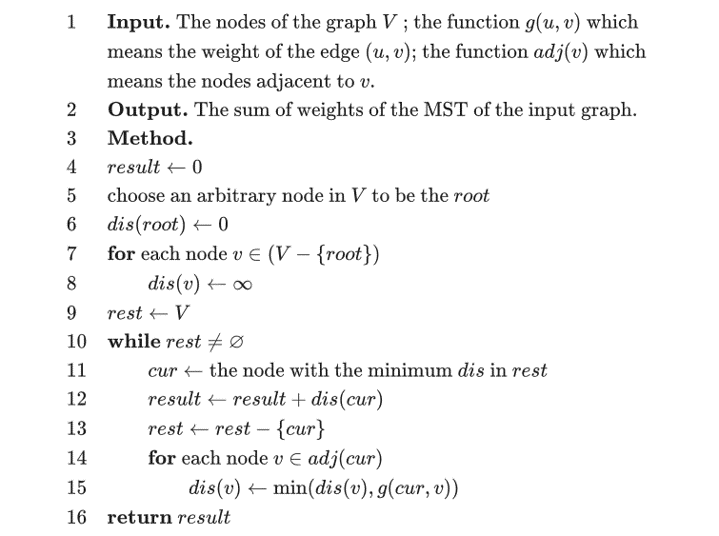
\includegraphics[width=0.7\textwidth]{assets/prim_pcode.png}
    \caption{prim算法的伪代码}
    \label{fig:prim_pcode}
\end{figure}

分析这个过程,在应用Prim算法的过程中,每次加入一个点,一共会加入$N$轮,每轮中需要找到一个距离已有点最小的点,使用遍历的方式查找,时间复杂度为 $O(N)$,同时每个点会更新它的邻边,每条边会被两个点更新两次,因此总的所有点更新边的时间复杂度为 $O(M)$。因此Prim算法的\textbf{时间复杂度}为 $O(N^2+M)$。

空间上需要存储整个图,\textbf{空间复杂度}为 $O(N+M)$。

\subsection{Prim+堆优化}

Prim堆优化算法是在Prim的基础上进行了改进,
我们可以看到在Prim算法的时间复杂度上,$O(N^2)$ 占据了较大的比例,而它的来源是每一次的查找最大值,
因此Prim堆优化就是使用堆来找到最大值。
每次用边更新节点时,会将如果更新了结点的值,则会将更新的结点的距离加入堆中,因此堆的大小与边数有关,为 $O(M)$。
每次更新的时间是 $O(\log M)$的,每条边都可能会进行一次,因此\textbf{时间复杂度}为 $O(M\log M)$。

而在每次通过堆获得最小值时,时间复杂度为 $O(\log M)$,共进行N轮,
因此总的时间复杂度为 $O(N\log M + M\log M)$,
因为堆的空间复杂度为 $O(M)$,因此\textbf{空间复杂度}仍为 $O(N+M)$。



\subsection{Kruskal算法}

Kruskal 算法是一种常见并且好写的最小生成树算法,由 Kruskal 发明\cite{RN2}。该算法的基本思想是从小到大加入边,是一个贪心算法。

\begin{figure}[htbp]
    \centering
    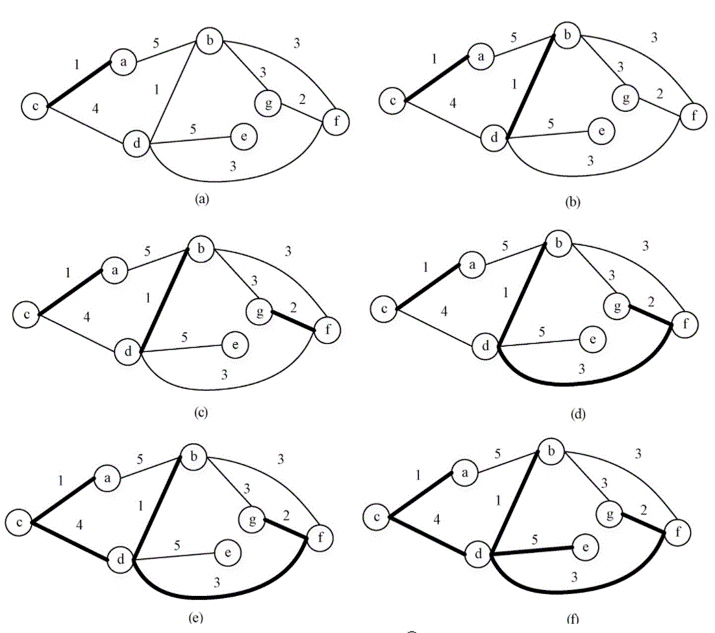
\includegraphics[width=0.5\textwidth]{assets/kruskal.png}
    \caption{Kruskal算法实例}
    \label{fig:kruskal}
\end{figure}


算法虽简单,但需要相应的数据结构来支持。具体来说,维护一个森林,查询两个结点是否在同一棵树中,连接两棵树。
抽象一点地说,维护一堆 集合,查询两个元素是否属于同一集合,合并两个集合。
其中,查询两点是否连通和连接两点可以使用并查集维护。

Kruskal算法的时间复杂度瓶颈在于排序算法,使用快速排序、归并排序等算法进行排序,时间复杂度为$O(M\log M)$。在之后的并查集中,最坏进行M轮判定,每次判定两个结点是否连通需要$O(\alpha(N))$。就可以得到\textbf{时间复杂度}为$O(M\log M+M\alpha(M,N))$的Kruskal算法。



伪代码如下:
\begin{figure}[htbp]
    \centering
    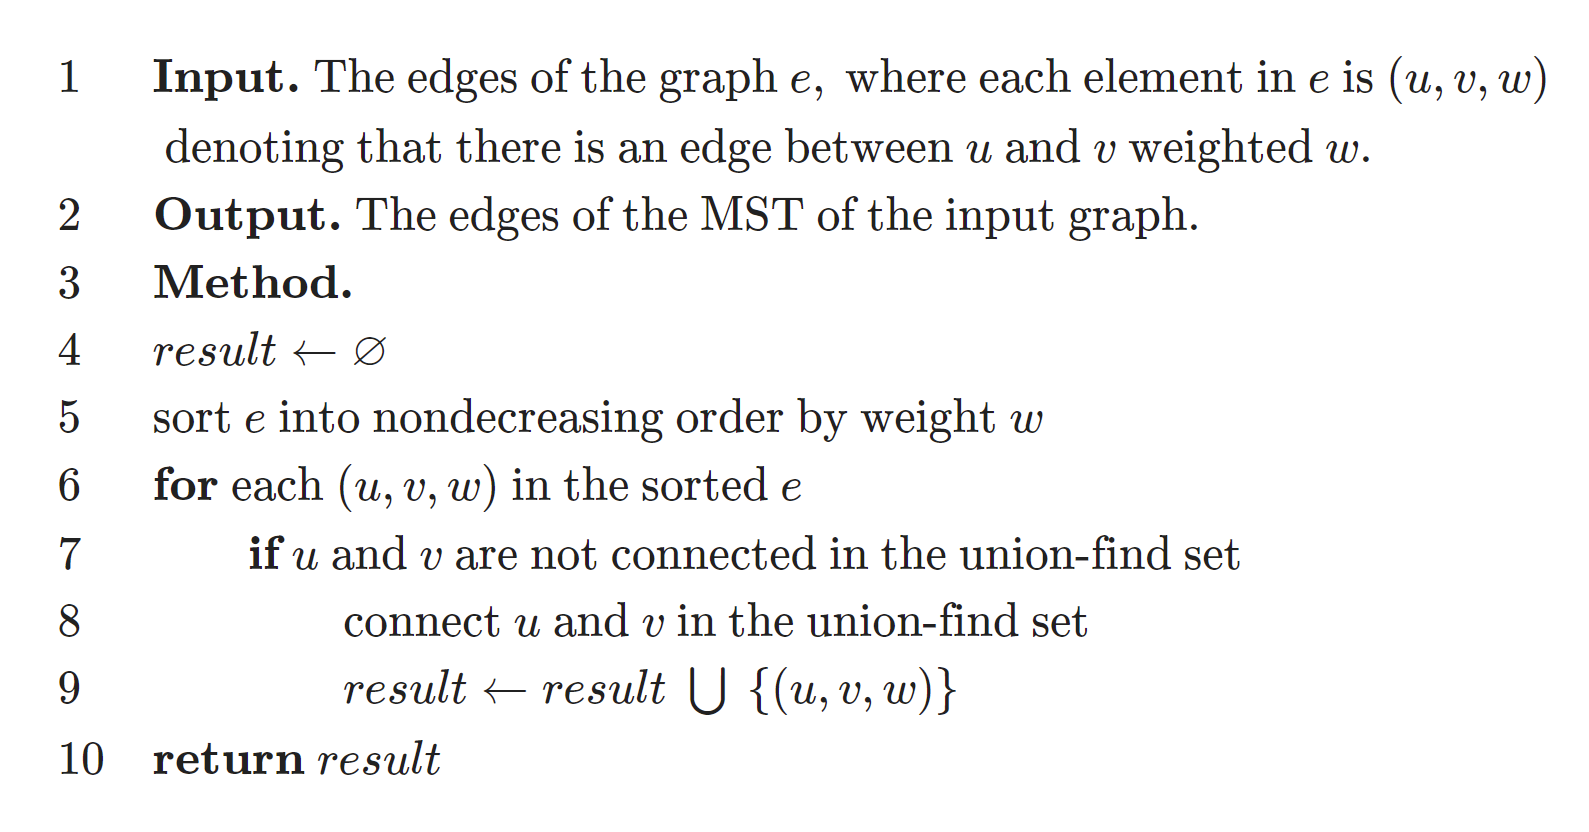
\includegraphics[width=0.6\textwidth]{assets/kruskal_pcode.png}
    \caption{Kruskal算法的伪代码}
    \label{fig:kruskal_pcode}
\end{figure}

并查集空间复杂度为 $O(N)$ \textbf{空间复杂度}为 $O(N+M)$。


在最小生成树的问题中,通常我们有$N<M<N^2$ 因此带入关系,我们总结上述算法可以得到表\ref{tab:comp}

\begin{table}[htbp]
    \centering
    \begin{tabular}{|l|l|l|l|}
    \hline
          & Prim & Prim堆优化 & Kruskal \\ \hline
    时间复杂度 &  $O(N^2)$    &     $O(M\log M)$    &     $O(M\log M)$    \\ \hline
    空间复杂度 &  $O(M)$      &     $O(M)$          &     $O(M)$          \\ \hline
    \end{tabular}
    \caption{几种算法的复杂度分析}
    \label{tab:comp}
\end{table}



其中Prim堆优化和Kruskal虽然都是$O(M\log M)$,但是Prim堆优化中只有更新了距离值的边才会加入堆中,因此这个$M$的值是会十分小的,尤其是在等权的情况下。
而Kruskal的$M$则是固定为图中的边数$M$,如果使用快速排序,其复杂度甚至可能在$O(M\log M)$到$O(M^2)$间摆动


\section{实验设计}\label{ss:design}
为了验证我们在\ref{sec:theo}中给出的分析结论,我们完成如下的实验验证。实验中的计算机为Ubuntu 16.04.6 LTS (GNU/Linux 4.4.0-142-generic x86\_64) 48核。

在我们的实验中,我们设计了生成边权的程序,生成图的程序,运行实验的脚本,以及实验用的Kruskal和Prim程序。

关于不同算法的评测,我们使用了C语言的时间计算库<sys/time.h>中的gettimeofday() 函数计量时间。精确到微秒(\(10^{-6}s\)),忽略读入时间,测试10次取平均值。

\begin{lstlisting}[language=c]
double get_time(){
	struct timeval tv;
	double t;
	gettimeofday(&tv, (struct timezone *)0);
	t = tv.tv_sec + (double)tv.tv_usec * 1e-6;
	return t;
}
\end{lstlisting}

我们在实验中要验证三类因素的影响,固定节点数情形下稀疏程度的影响,添加边不同方式的影响,边权生成方式的影响。

首先,图的节点个数必然和总耗时是正比的,节点个数越多,总耗时越大。我们对图的分类可以根据节点数的大小进行分类,来验证稀疏程度和加边方式的影响。我们的实验验证从100到1000,以100为步长,来实现对于我们工程的正确性的验证。
随后我们以2000位为步长,从2000到20000遍历完成更大规模的实验验证。

\noindent\textbf{稀疏程度的验证}\quad 从而分析不同稀疏程度对于两个算法的影响。然后我们考虑在N个节点的图中,我们考虑边的数量,这里我们比较容易想到两种特殊的图,它们分别代表了稀疏图和稠密图的极端情况:

a.N个节点的最小连通情况 –-树

b.N个节点之间相互都连有边 –- 完全图

这两种情形通常出现在N较大的情况中,不适合进行分步加边,在这种情况下我们使用的是vector进行存储,只有vector才能支持N=20000,M=199990000的存储。

这种情况下只需要读入边权,然后构建一棵树输出,完全图则只需要两个for循环判断两个节点不相同就相连就可以

\begin{lstlisting}
// 生成完全图
// 枚举左节点
for u from 1 to n
    // 枚举右节点
    from v from u + 1 to n
    add_edge(u, v)
\end{lstlisting}

这里构建树的方法非常简单,即对第i个节点,随机一个节点j (j < i),然后将他们连通,这样就能保证每个节点连通,而且没有环,因为前面的节点不可能有回边。
\begin{lstlisting}
// 生成树
// 枚举左节点
for u from 2 to n
    // 枚举一个[1, u-1]内的随机数作为右节点
    v = rand() % (u-1) + 1
    add_edge(u, v)
\end{lstlisting}


\noindent\textbf{加边方式}\quad 我们想到可以通过加边的形式来从树变成完全图,这里我们根据Prim和Kruskal算法集中式和分布式地构建其最小生成树的方式,想到了两种方法。第一种是\textbf{平均}地在图上加边,每次数目固定。我们从每个点的度数入手实现平均加边,因为最后一个完全图的所有点的度数都为n-1,那么在加边的第T轮,我们只给度数<T的节点之间连边,这样就可以让整个图平均加边,这样只需要进行n-1轮,所有的节点就都相互连通。

\begin{lstlisting}
// 平均方式加边
function::add_average(T)
//枚举左节点
    for u from 1 to n
        //选择度数小于T的节点加边
        if deg[u] < T
            for v from 1 to n
                //找到一个度数小于T,不曾连过边的不同节点连接
                if deg[v] < T and !connect(u, v) and u != v
                    add_edge(u, v)
                    //一个节点只主动加一条
                    break
\end{lstlisting}

另一种,基于我们对Prim算法的思考,我们使用了\textbf{集中加边}:由于Prim的生成过程是从一个点开始依次寻找最近节点,所以我们猜测以每个点都加满的星状图会对Prim有利。我们从每个节点入手,直接让这个节点与所有的节点连边,这样我们执行n-1轮,也就让这个图变成完全图了。
\begin{lstlisting}
//集中方式加边
function::add_pernode(T)
    //第T次就把第T个节点给补满
    u = T
    for v from 1 to n
        //找到所有u没有连接的节点都连接
        if u != v and !connect(u,v)
            add_edge(u, v)
\end{lstlisting}

\noindent\textbf{边权的生成}\quad 由于Kruskal的算法瓶颈在于排序算法,而排序算法会受到一些边界情况的影响,所以我们构建了如下三种生成方式对新添加的边进行权值分配:
\begin{itemize}
    \item 等权:直接令所有边的权值为1
    \item 随机:所有边的权值随机,使用<cstdlib>库中的伪随机数获取(1,m)之间的随机数
    \item 排列:所有边的权值不相同,构造数组,然后调用<algorithm>中的random\_shuffle函数
\end{itemize}

实验中我们编写了测试shell脚本,根据设置的节点大小,自动执行我们的测试任务。
\begin{lstlisting}
枚举节点N   
	根据N得到M
    并根据M生成边权
    枚举不同的边权
        根据当前边权生成图
		枚举不同的图
			枚举进行的轮数
				根据当前的图执行prim
			计算平均值
			枚举进行的轮数
				根据当前的图执行kruskal
			执行平均值
\end{lstlisting}

\section{实验过程和结果分析}
\subsection{工程正确性验证}
在\ref{ss:design}中我们已经说到,我们先使用较少的节点进行正确性验证,这里基于Jupyter Notebook进行快速的原型迭代,确认获得了正确的实验数据。如图\ref{fig:100a}
\begin{figure}[htbp]
    \centering
    \subfigure[100节点等权]{
        \begin{minipage}[t]{0.45\linewidth}
            \centering
            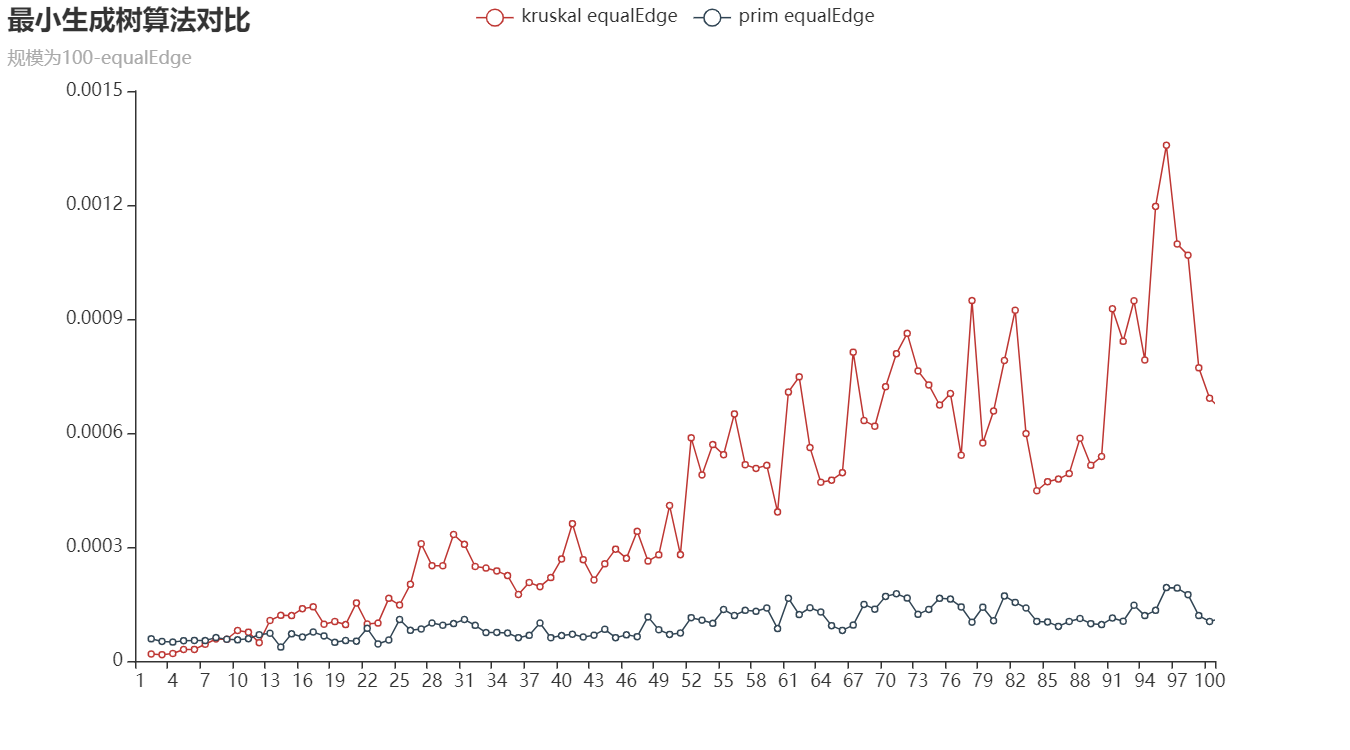
\includegraphics[width=0.95\textwidth]{assets/100节点-等权-不同稀疏度.png}
        \end{minipage}
    }
    \subfigure[100节点排列权]{
        \begin{minipage}[t]{0.45\linewidth}
            \centering
            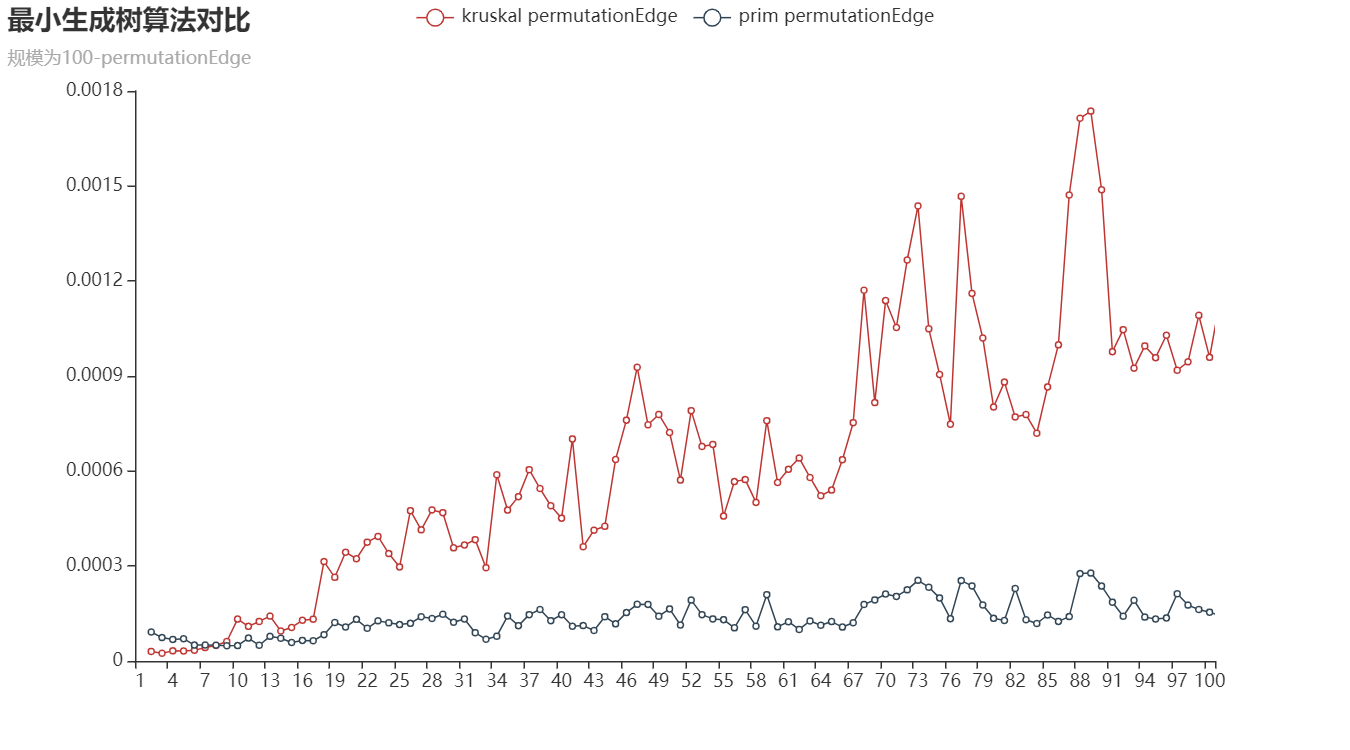
\includegraphics[width=0.95\textwidth]{assets/100节点-排列权-不同稀疏度.png}
        \end{minipage}
    }
    
    \subfigure[100节点随机权]{
        \begin{minipage}[t]{0.45\linewidth}
            \centering
            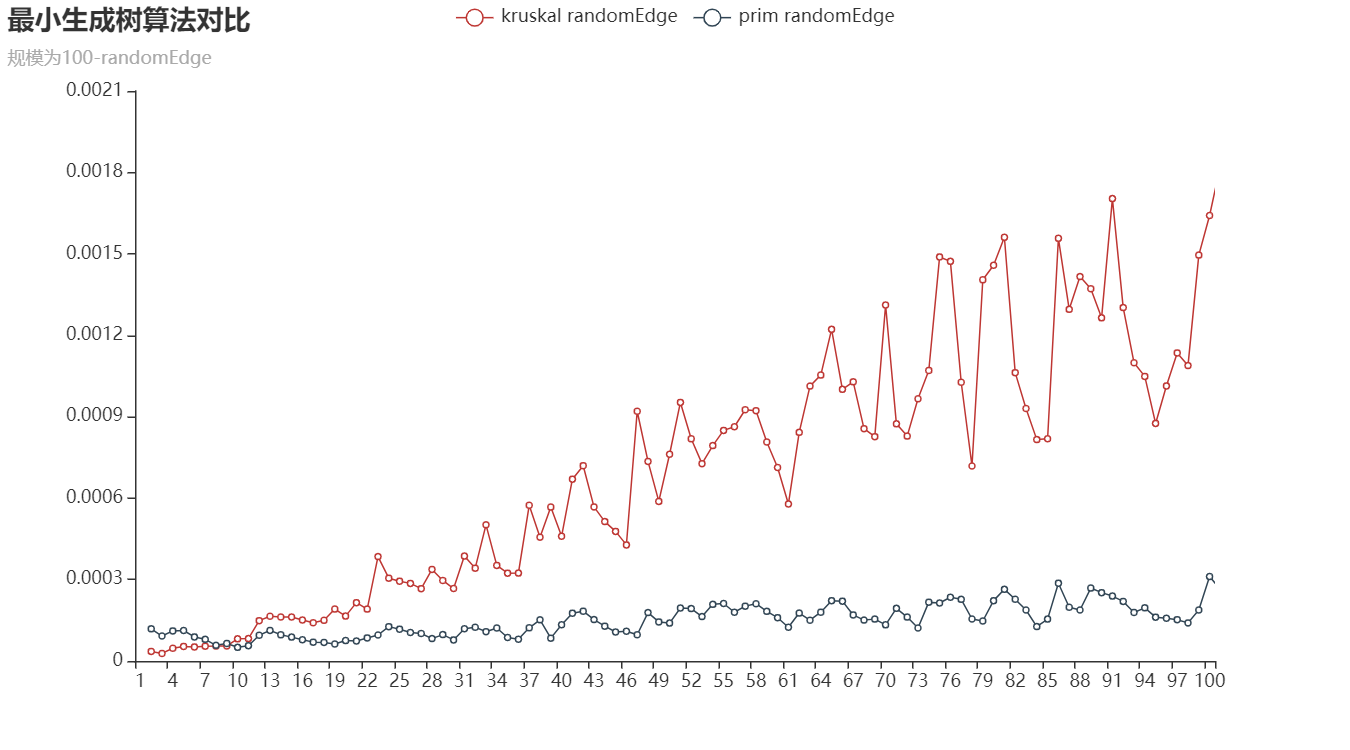
\includegraphics[width=0.95\textwidth]{assets/100节点-随机权-不同稀疏度.png}
        \end{minipage}
    }
    \caption{100节点}
    \label{fig:100a}
\end{figure}

我们首先测定了100节点下,Prim和Kruskal两种算法的不同权值分配方式对应的稀疏度的影响图线如图\ref{fig:100a}

实验结果符合预期,即Kruskal对于边数敏感,随着边数增多,耗时显著增加。对于Prim来说,由于节点数确定,大体上的耗时没有非常显著的变化。

但是我们在这里发现了一个问题,即便是对于100这样的少节点数情况,我们添加了少量边之后,仍然表现出稠密图的性质,使得Kruskal表现极差。这给我们了一个指导,即在当前的加边方式之下,可以将观察的重点放到较为稀疏的区间上,这样才能较为完整地展现稀疏图Kruskal更优的特性。

另外我们发现,三种权值分配方式的耗时依次递增如下:等权、排列权、随机权。这和Kruskal中使用到排序有关;另外,这和我们设定的权值大小有关,由于等权的情形中,我们设定所有边全为1,所以比起另外两种有较大权值的情况,应当在算术、读写等多方面都会更快。

我们在验证部分中还研究了200节点和500节点的情形,如图\ref{fig:200&500a}
\begin{figure}[htbp]
    \centering
    \subfigure[200节点等权]{
        \begin{minipage}[t]{0.45\linewidth}
            \centering
            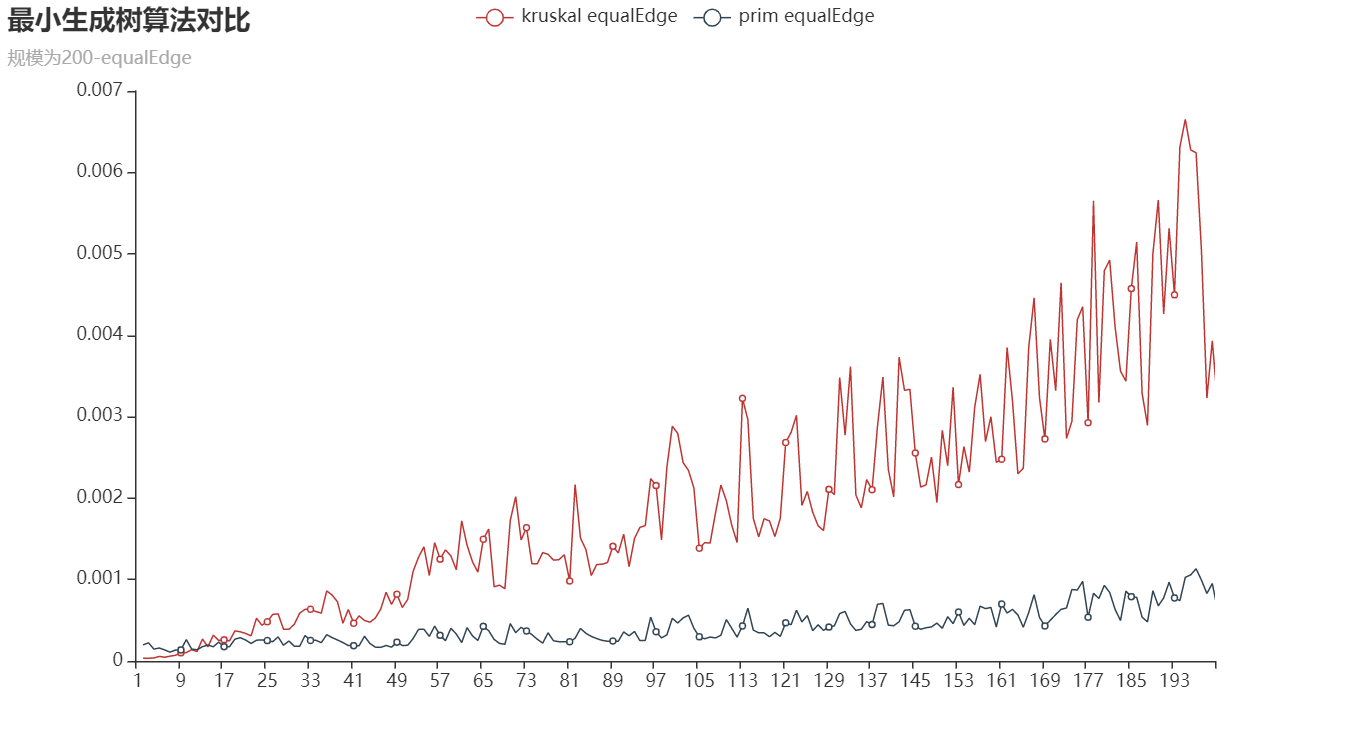
\includegraphics[width=0.95\textwidth]{assets/200节点-等权-不同稀疏度.png}
        \end{minipage}
    }
    \subfigure[200节点排列权]{
        \begin{minipage}[t]{0.45\linewidth}
            \centering
            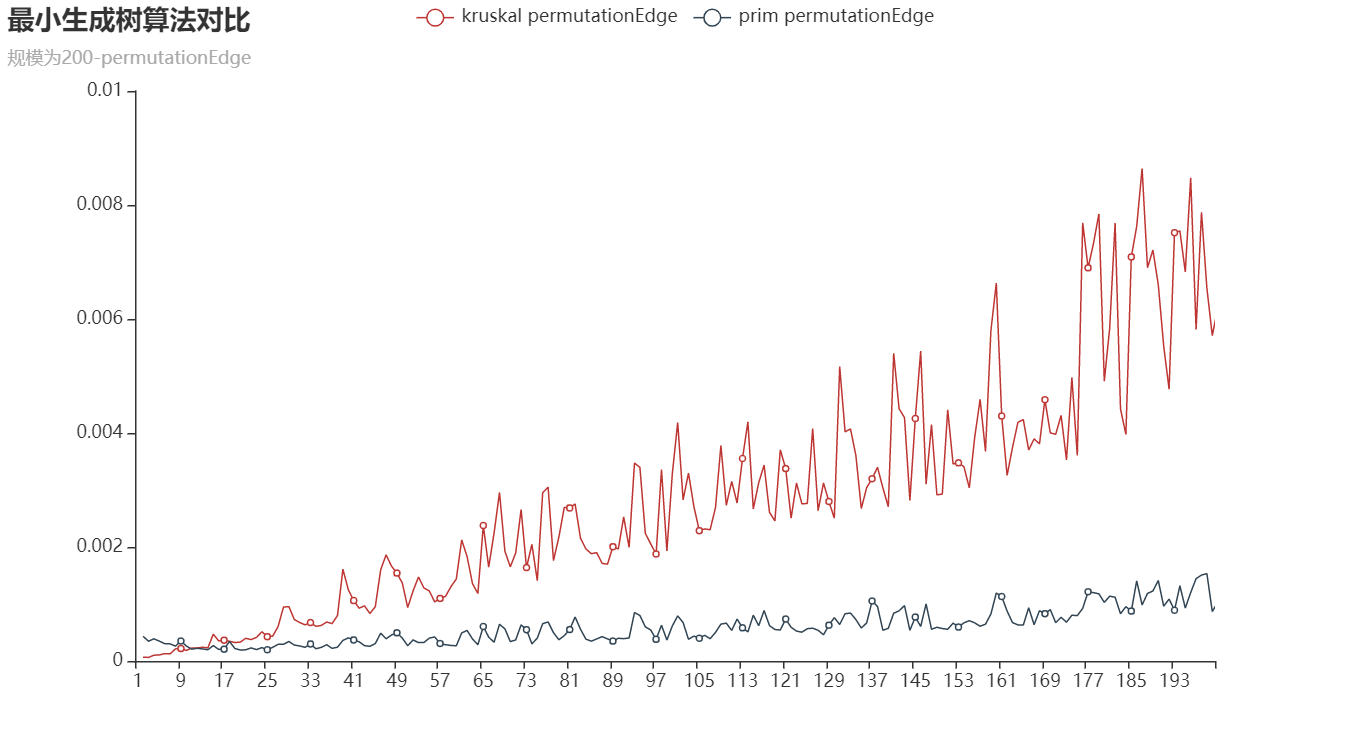
\includegraphics[width=0.95\textwidth]{assets/200节点-排列权-不同稀疏度.png}
        \end{minipage}
    }

    \subfigure[200节点随机权]{
        \begin{minipage}[t]{0.45\linewidth}
            \centering
            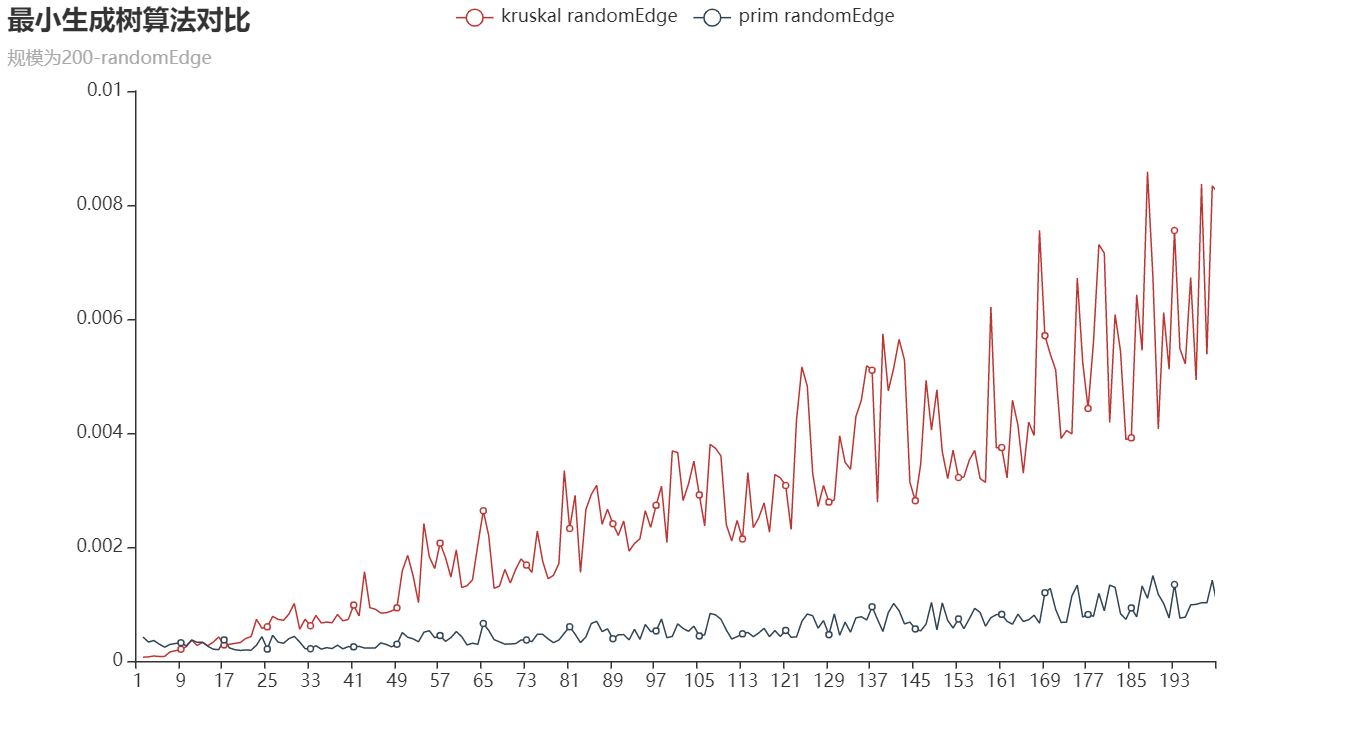
\includegraphics[width=0.95\textwidth]{assets/200节点-随机权-不同稀疏度.png}
        \end{minipage}
    }
    \subfigure[500节点等权]{
        \begin{minipage}[t]{0.45\linewidth}
            \centering
            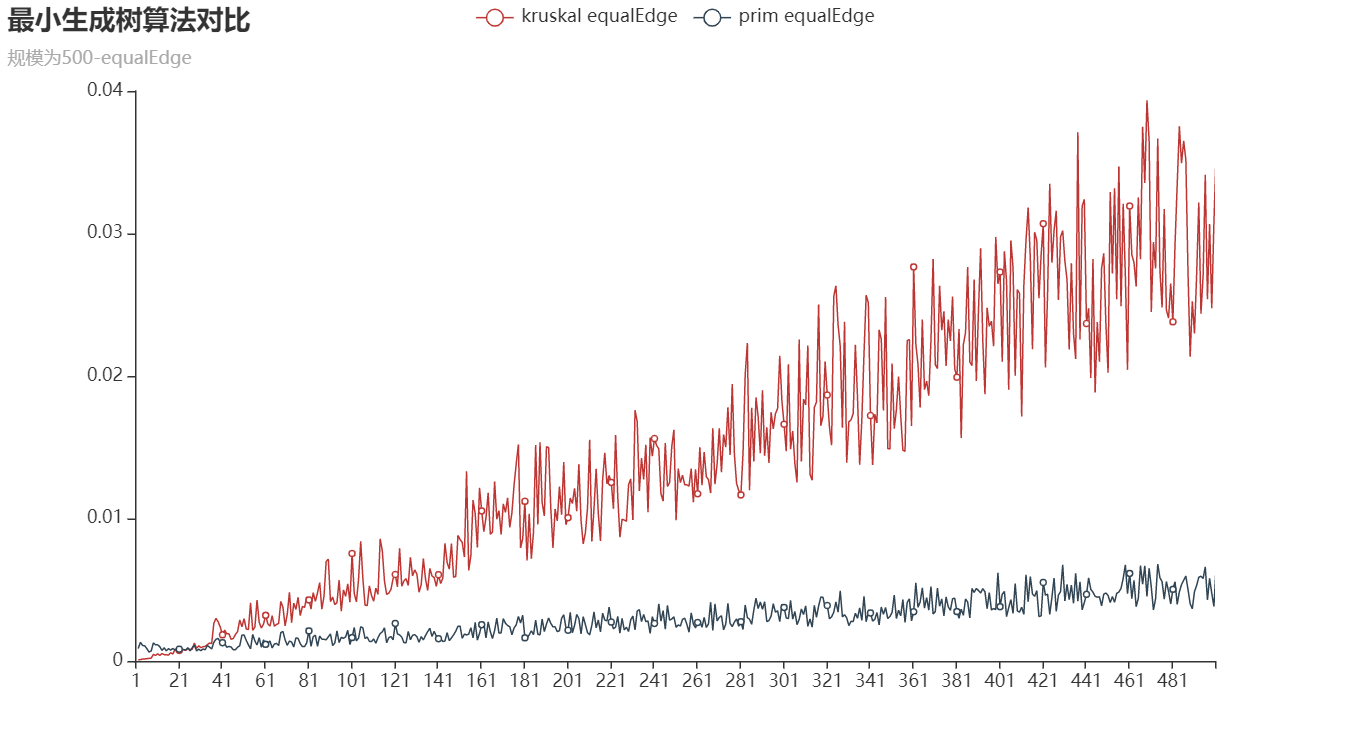
\includegraphics[width=0.95\textwidth]{assets/500节点-等权-不同稀疏度.png}
        \end{minipage}
    }

    \subfigure[500节点排列权]{
        \begin{minipage}[t]{0.45\linewidth}
            \centering
            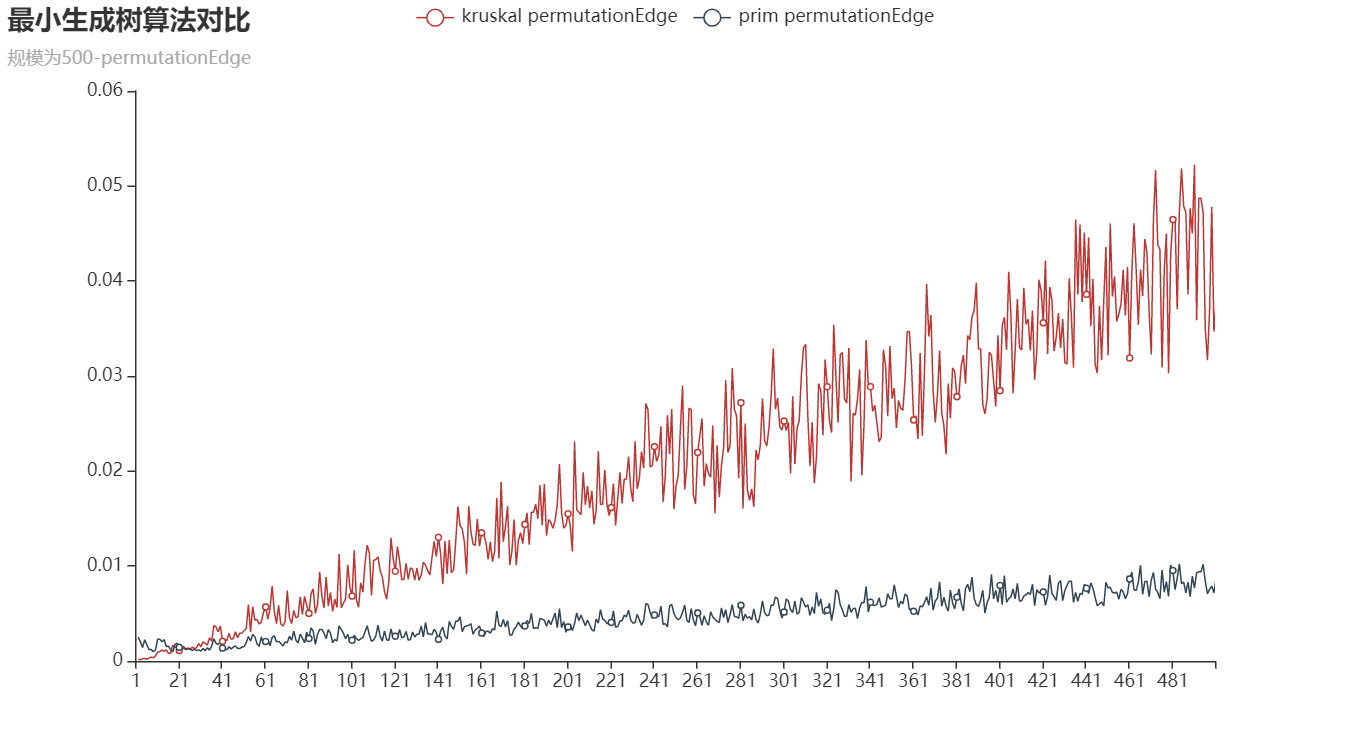
\includegraphics[width=0.95\textwidth]{assets/500节点-排列权-不同稀疏度.png}
        \end{minipage}
    }
    \subfigure[500节点随机权]{
        \begin{minipage}[t]{0.45\linewidth}
            \centering
            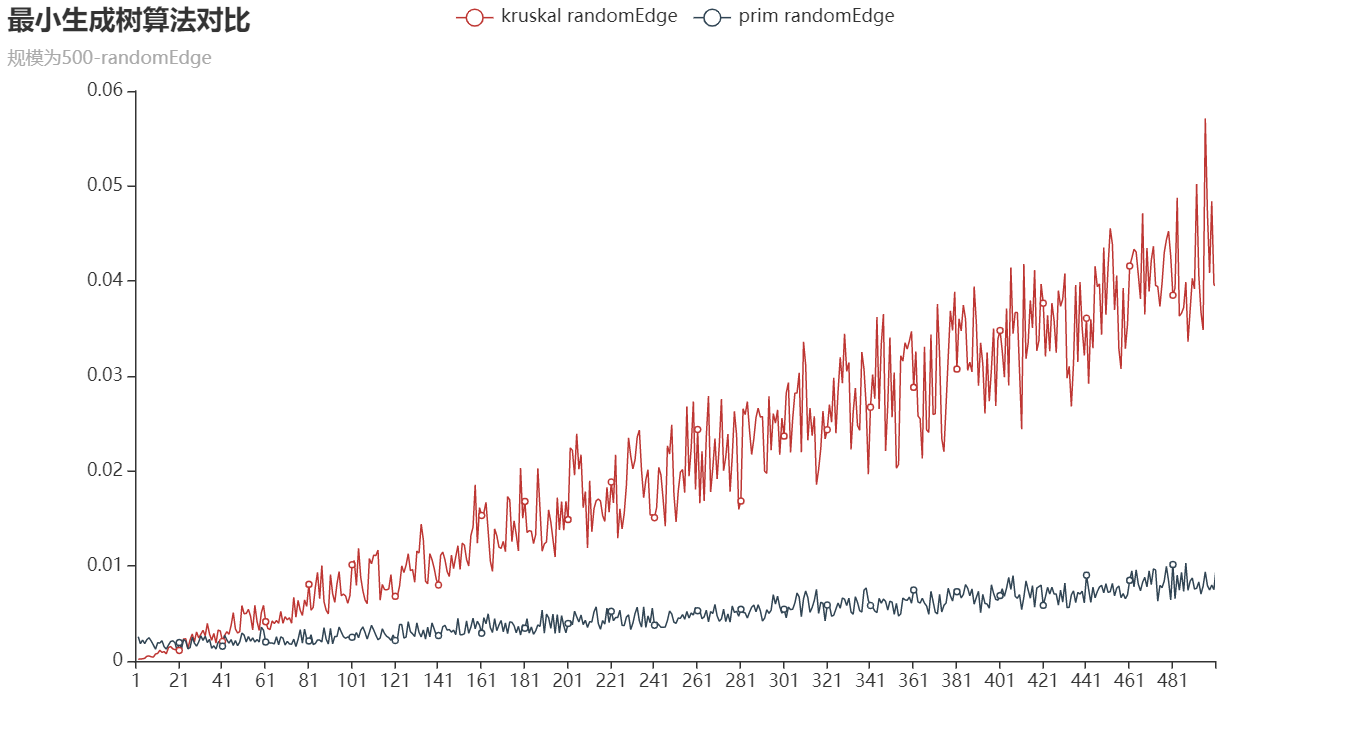
\includegraphics[width=0.95\textwidth]{assets/500节点-随机权-不同稀疏度.png}
        \end{minipage}
    }
    \caption{更多的验证}
    \label{fig:200&500a}
\end{figure}

\subsection{Prim堆优化算法的验证}
在\ref{sec:theo}中我们给出了几种算法的复杂度分析,从中,我们可以抽象地看到Prim堆优化算法的优势,于是,我们在1000节点下进行了关于时间消耗关于复杂度的可视化,如图\ref{fig:primheap},三幅图分别对应不同的权值生成方式:
\begin{figure}[htbp]
    \centering
    \subfigure[等权]{
        \begin{minipage}[t]{0.45\linewidth}
            \centering
            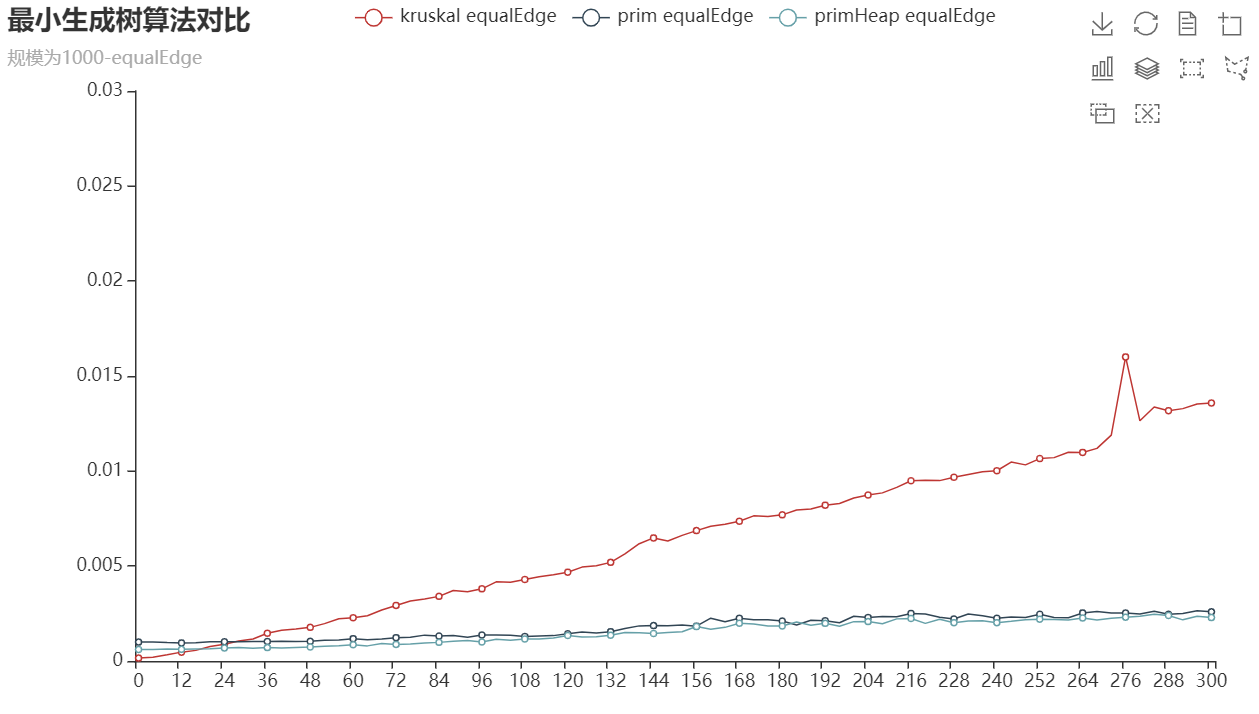
\includegraphics[width=0.95\textwidth]{assets/堆优化-等权.png}
        \end{minipage}
    }
    \subfigure[排列权]{
        \begin{minipage}[t]{0.45\linewidth}
            \centering
            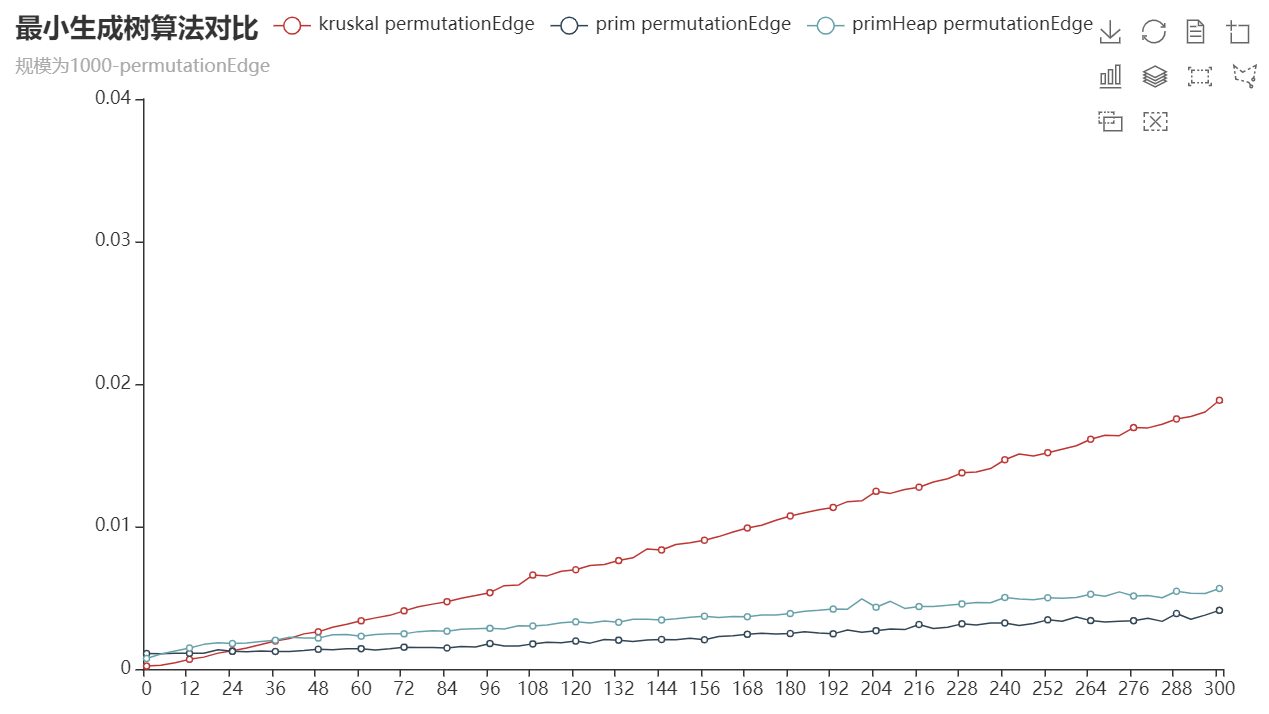
\includegraphics[width=0.95\textwidth]{assets/堆优化-排列权.png}
        \end{minipage}
    }
    
    \subfigure[随机权]{
        \begin{minipage}[t]{0.45\linewidth}
            \centering
            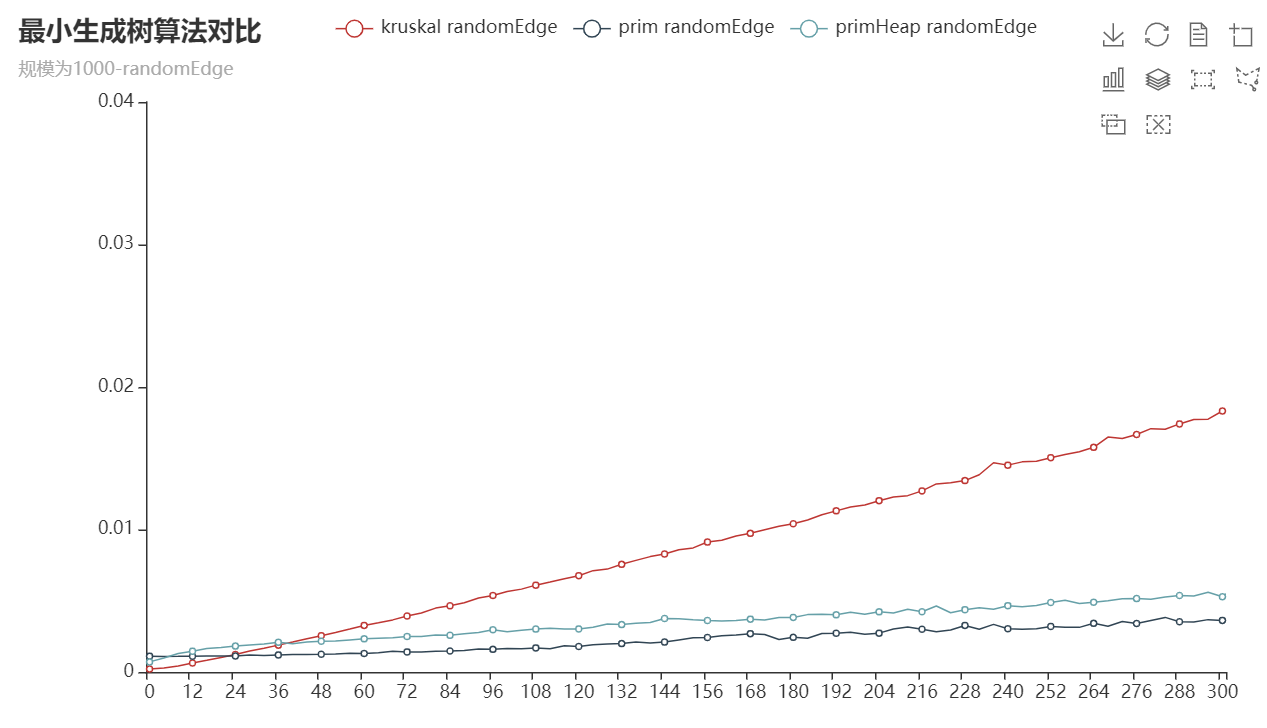
\includegraphics[width=0.95\textwidth]{assets/堆优化-随机权.png}
        \end{minipage}
    }
    \caption{堆优化Prim具有鲜明的优势}
    \label{fig:primheap}
\end{figure}

数据也可以佐证这种观点,如表\ref{tab:primheap}中给出了前30次加边的数据,可以看到带有堆优化的Prim算法比前两者有1到4个量级的显著优势:
\begin{table}[htbp]
    \begin{tabular}{|c|c|c|c|}
    \hline
    加边次数 & kruskal permutationEdge & prim permutationEdge & primHeap permutationEdge \\ \hline
    0    & 0.000282836             & 0.004374313          & 0.000012009              \\ \hline
    2    & 0.0003677845            & 0.004419255          & 0.0000407862             \\ \hline
    4    & 0.0006066561            & 0.004230952          & 0.0000827002             \\ \hline
    6    & 0.0009082079            & 0.003866029          & 0.000025091              \\ \hline
    8    & 0.001223993             & 0.003810096          & 0.0000326012             \\ \hline
    10   & 0.001528716             & 0.003810287          & 0.0000584934             \\ \hline
    12   & 0.001880312             & 0.003765082          & 0.0000629042             \\ \hline
    14   & 0.00225513              & 0.003938484          & 2.882e-7                 \\ \hline
    16   & 0.002473497             & 0.003872943          & 0.0000722025             \\ \hline
    18   & 0.002831554             & 0.003915191          & 0.0000825022             \\ \hline
    20   & 0.003151321             & 0.004017734          & 0.0000898932             \\ \hline
    22   & 0.003507113             & 0.004193521          & 0.0000292084             \\ \hline
    24   & 0.003890133             & 0.00421176           & 0.0000093004             \\ \hline
    26   & 0.00420382              & 0.004409122          & 0.0000298998             \\ \hline
    28   & 0.00466578              & 0.004312968          & 0.000046899              \\ \hline
    30   & 0.004886341             & 0.004360104          & 0.0000530025             \\ \hline
    \end{tabular}
    \caption{三种算法的对比}
    \label{tab:primheap}
\end{table}

在我们所设定的多种条件下,带有堆优化的Prim算法都是完胜的,所以在更详细的对比中,出于计算资源和时间等的考量,且为了让我们的对比实验更有意义,我们不再对带有堆优化的Prim算法进行探究。接下来的实验,如果没有特别说明,都是针对朴素Prim算法和Kruskal算法的对比实验。

\subsection{扩大节点数目}
基于之前关于选取观察区间和大概趋势的思考,这里我们对于2000、5000、10000三种情形的前200次加边的图进行最小生成树算法的对比。

结果是显然的,Kruskal更加适合较为稀疏的情形而Prim更加适合较为稠密的情形,如图\ref{fig:2000&5000a}和\ref{fig:10000a}:
\begin{figure}[htbp]
    \centering
    \subfigure[2000节点等权]{
        \begin{minipage}[t]{0.45\linewidth}
            \centering
            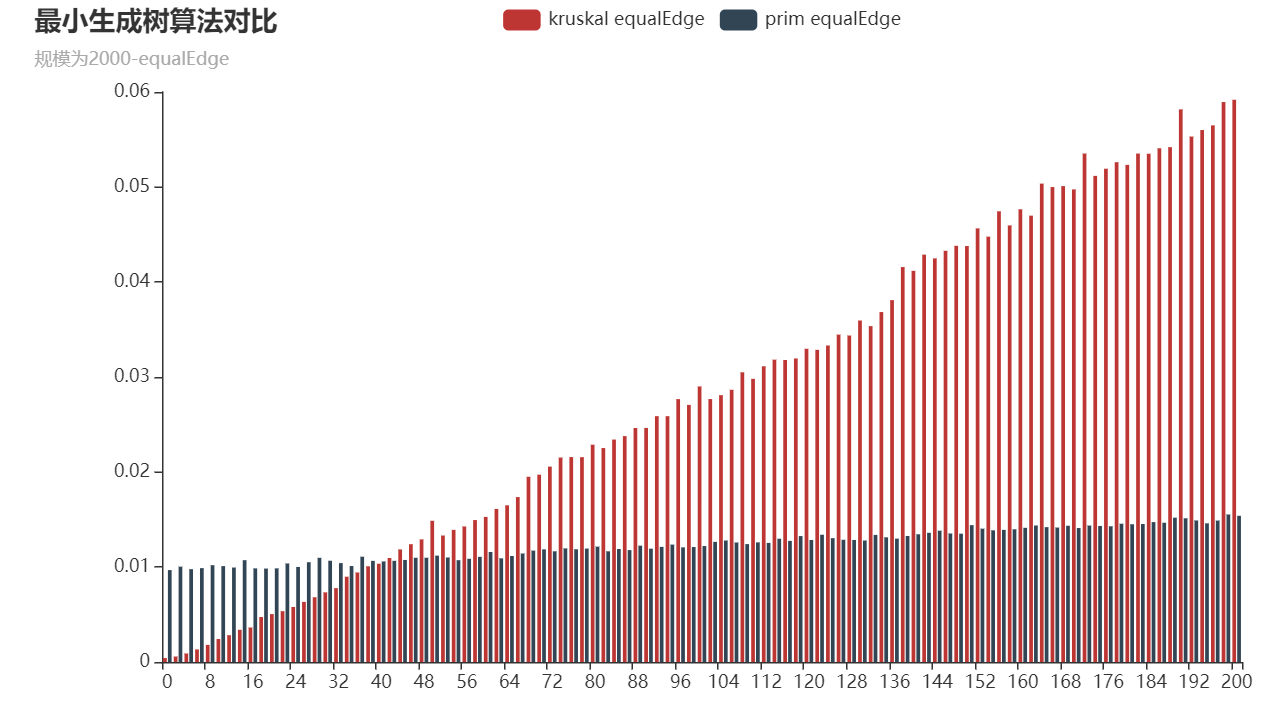
\includegraphics[width=0.95\textwidth]{assets/2000节点-等权-不同稀疏度.png}
        \end{minipage}
    }
    \subfigure[2000节点排列权]{
        \begin{minipage}[t]{0.45\linewidth}
            \centering
            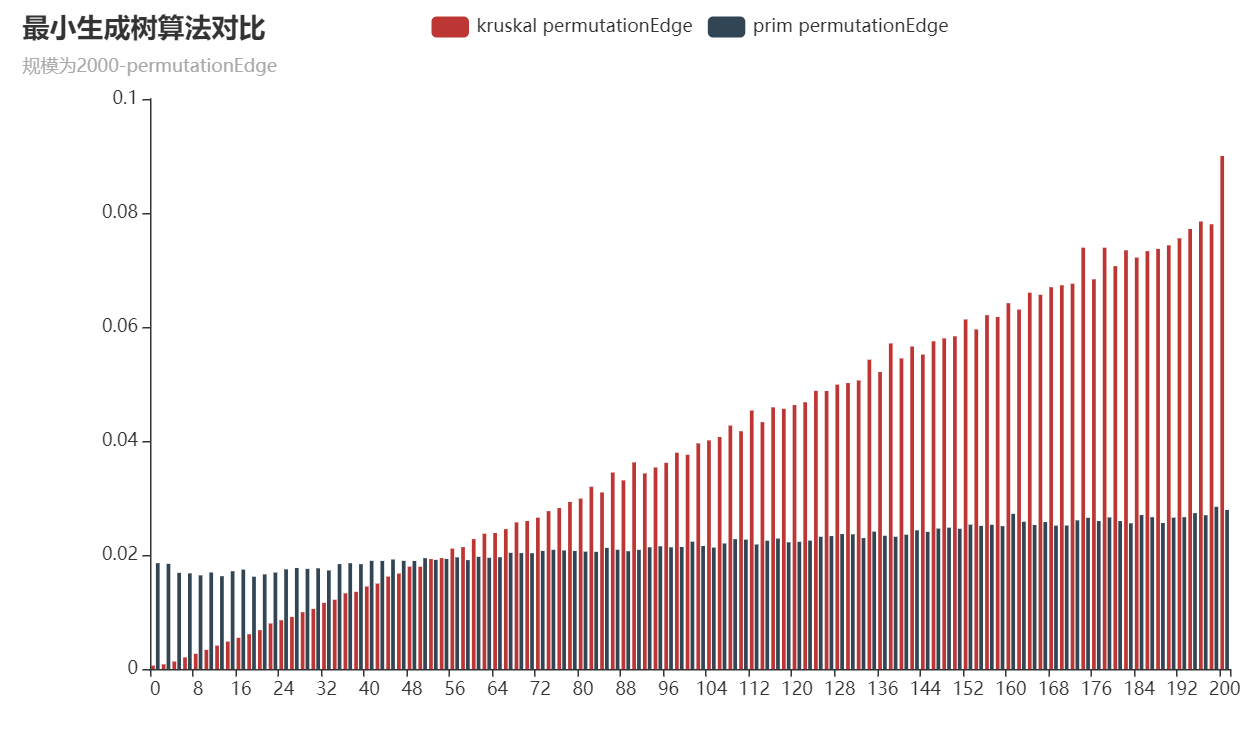
\includegraphics[width=0.95\textwidth]{assets/2000节点-排列权-不同稀疏度.png}
        \end{minipage}
    }

    \subfigure[2000节点随机权]{
        \begin{minipage}[t]{0.45\linewidth}
            \centering
            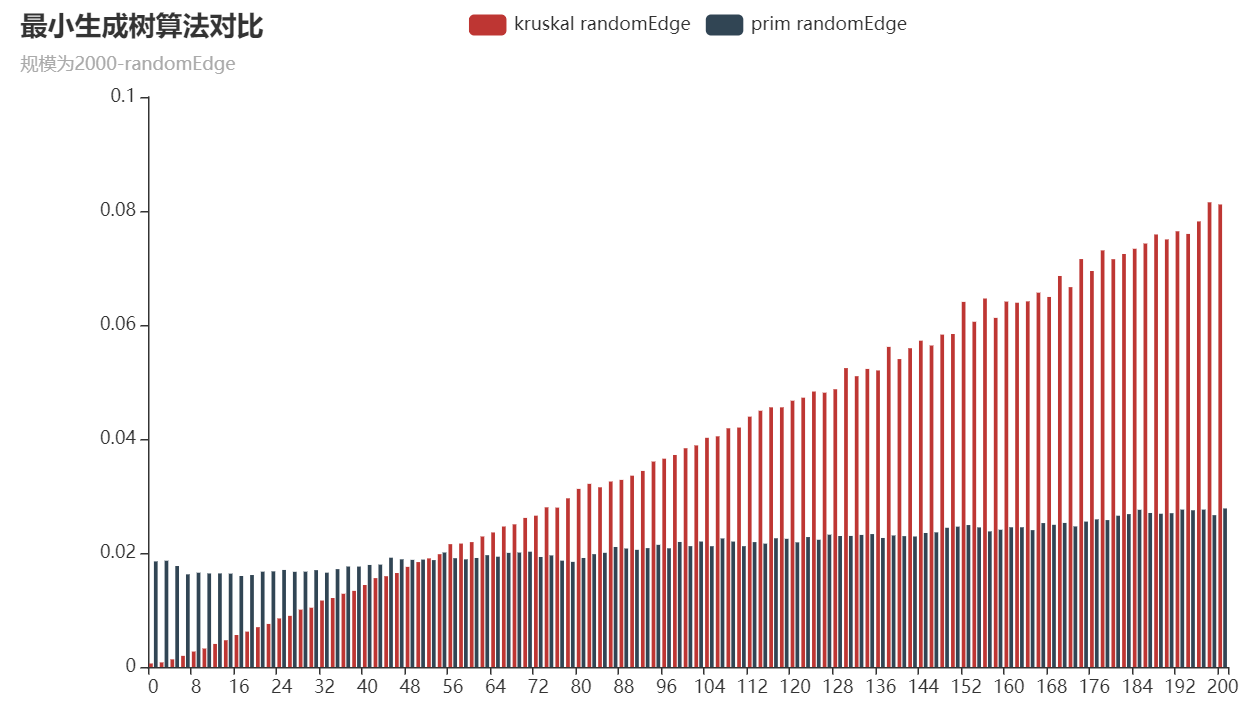
\includegraphics[width=0.95\textwidth]{assets/2000节点-随机权-不同稀疏度.png}
        \end{minipage}
    }
    \subfigure[5000节点等权]{
        \begin{minipage}[t]{0.45\linewidth}
            \centering
            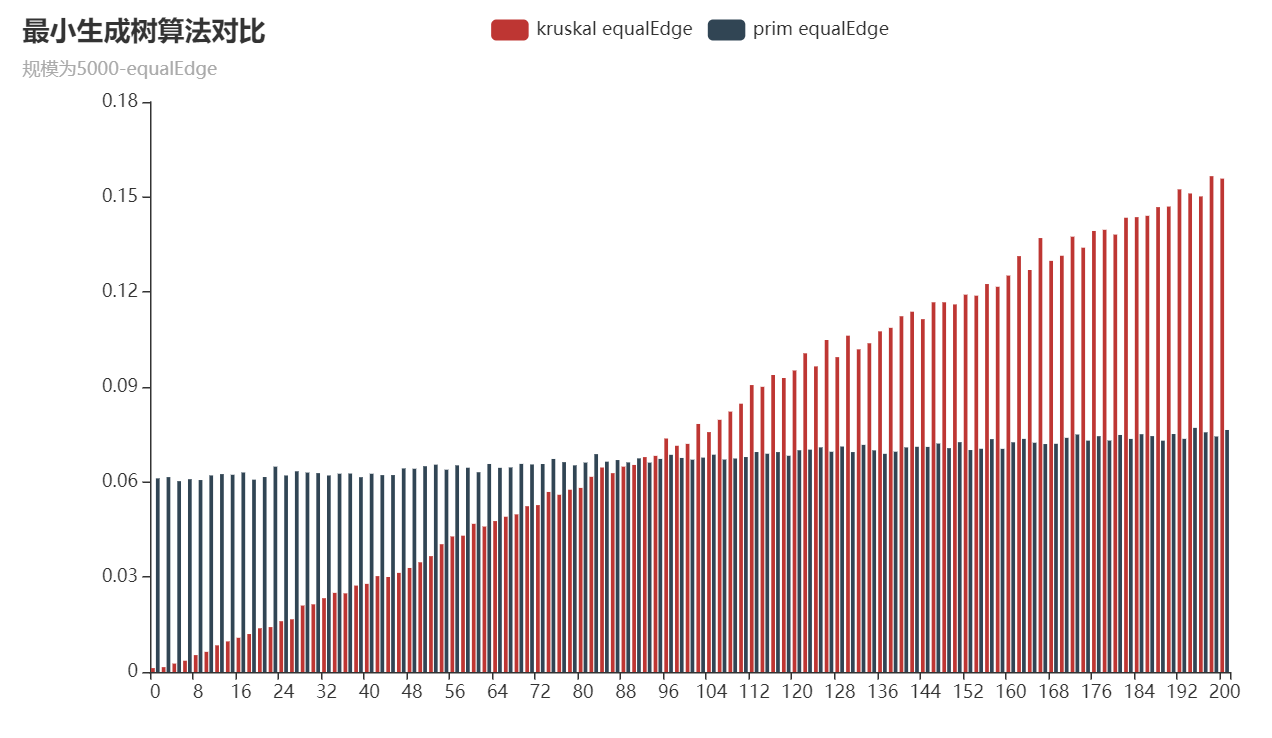
\includegraphics[width=0.95\textwidth]{assets/5000节点-等权-不同稀疏度.png}
        \end{minipage}
    }

    \subfigure[5000节点排列权]{
        \begin{minipage}[t]{0.45\linewidth}
            \centering
            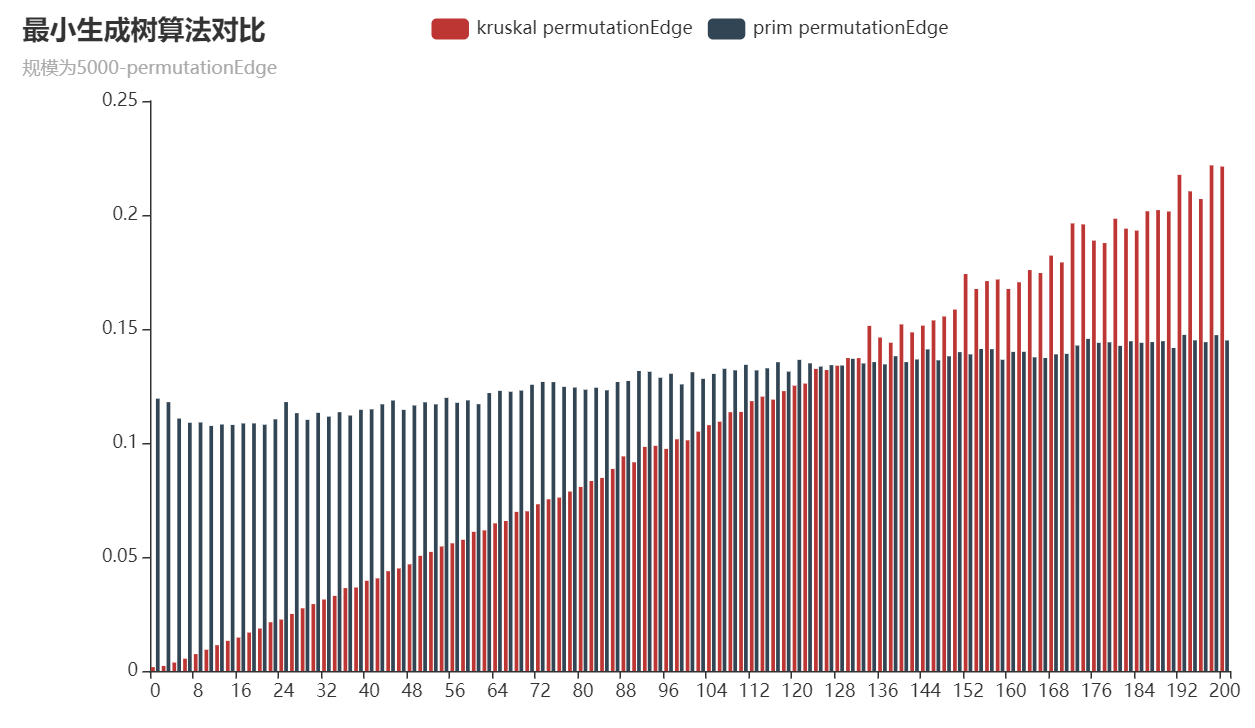
\includegraphics[width=0.95\textwidth]{assets/5000节点-排列权-不同稀疏度.png}
        \end{minipage}
    }
    \subfigure[5000节点随机权]{
        \begin{minipage}[t]{0.45\linewidth}
            \centering
            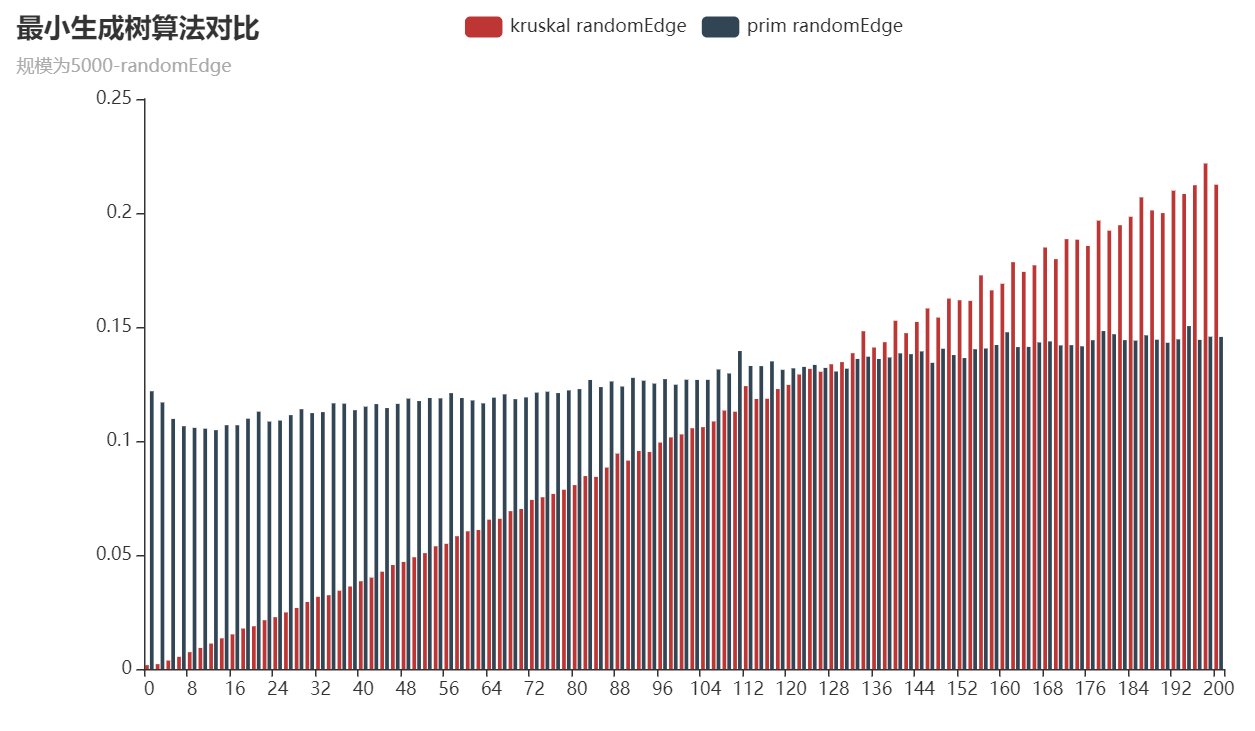
\includegraphics[width=0.95\textwidth]{assets/5000节点-随机权-不同稀疏度.png}
        \end{minipage}
    }
    \caption{较多节点数目情形的验证(1)}
    \label{fig:2000&5000a}
\end{figure}

我们把视角都聚焦在较小的范围,从而可以较为清晰地看到随着边数增多,Prim算法超过Kruskal算法的全过程。 另外,这个超越发生的点(我们成为超越点)在三个情形中并不相同,我们还能看出,对于同样加边次数的情形,节点数越高,超越点对应的加边次数越大。 

\begin{figure}[htbp]
    \centering
    \subfigure[10000节点等权]{
        \begin{minipage}[t]{0.45\linewidth}
            \centering
            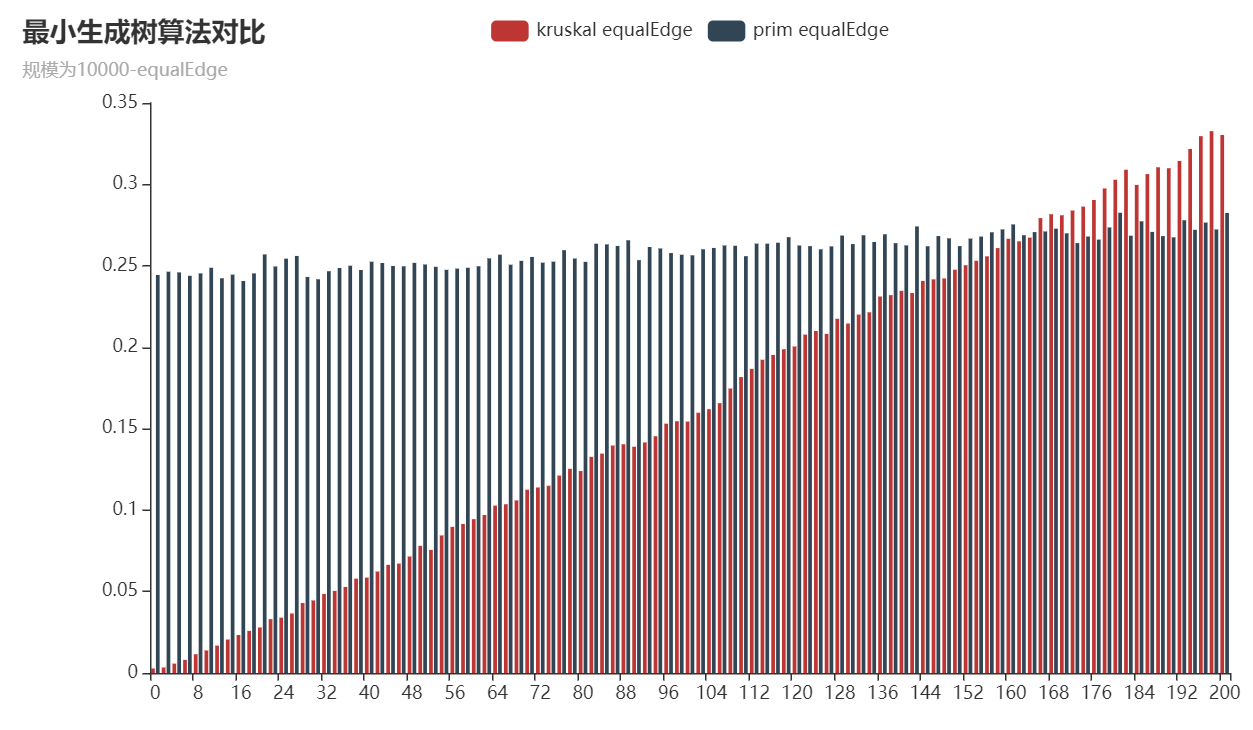
\includegraphics[width=0.95\textwidth]{assets/10000节点-等权-不同稀疏度.png}
        \end{minipage}
    }
    \subfigure[10000节点排列权]{
        \begin{minipage}[t]{0.45\linewidth}
            \centering
            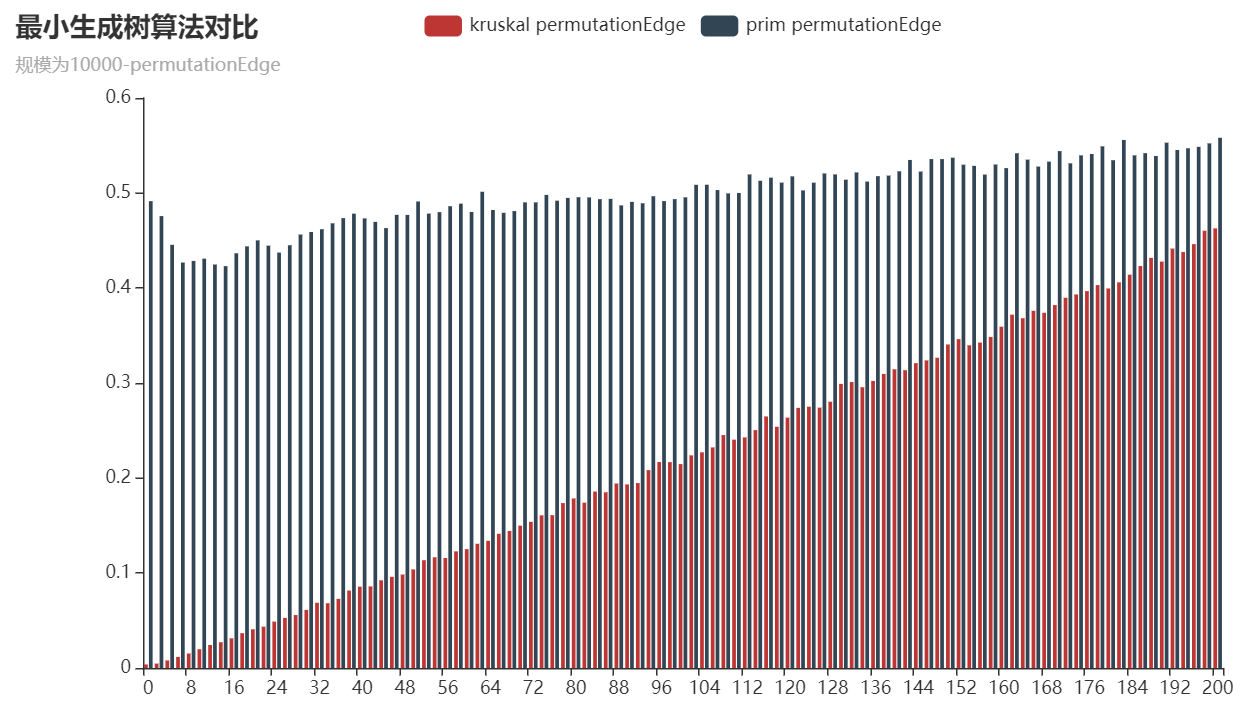
\includegraphics[width=0.95\textwidth]{assets/10000节点-排列权-不同稀疏度.png}
        \end{minipage}
    }
    \subfigure[10000节点随机权]{
        \begin{minipage}[t]{0.45\linewidth}
            \centering
            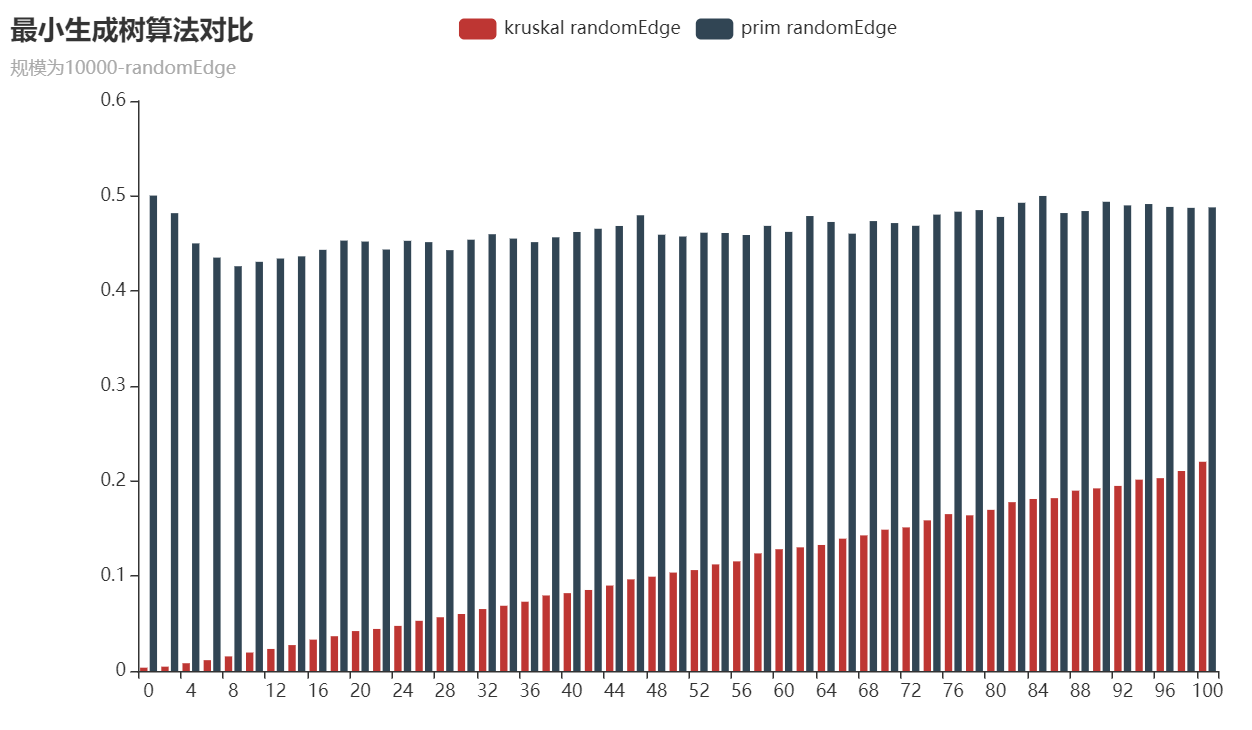
\includegraphics[width=0.95\textwidth]{assets/10000节点-随机权-不同稀疏度.png}
        \end{minipage}
    }
    \caption{较多节点数目情形的验证(2)}
    \label{fig:10000a}
\end{figure}

利用表\ref{tab:suppoint}的数据可以定性地看出这个对应加边次数和节点数正相关,且在较大的节点数下有较好的线性,对于等权的情况,斜率约为\(\frac{1}{50}\):

\begin{table}[htbp]
    \centering
    \begin{tabular}{|c|c|c|c|c|}
    \hline
    N    & 500  & 2000 & 5000  & 10000 \\ \hline
    等权   & 28   & 40   & 94    & 164   \\ \hline
    随机权  & 23   & 52   & 126   & /     \\ \hline
    排列权  & 21   & 52   & 128   & /     \\ \hline
    logN & 6.21 & 7.6  & 8.517 & /     \\ \hline
    \end{tabular}
    \caption{不同节点数、不同边权生成方式的超越点位置}
    \label{tab:suppoint}
\end{table}

\subsection{加边方式的对比}
在\ref{ss:design}中,我们描述了两种加边的方式,在如上的添加边的过程当中,我们作了平均加边。 但很自然地,我们有如下的思考:Prim算法是基于节点向外延展,而Kruskal算法是分布式地找边,随后连接节点,所以,将一个个节点依次加满的半满图,可能对于Prim算法的表现更加有利。

我们构建一系列实验情形,按照\ref{ss:design}中给出的单点集中加边的模式,构建星状图,对比两种MST算法的不同表现。需要注意的是,在我们的工作和可视化中,星状图、pernode、集中加边的意义是相同的,都是按照点集中加边,每次添加边数为\(n-1,n-2,\cdots,1,0\)依次减少。

我们验证了几个较少节点的情况,包括100,200,500,大体结果相同,这里使用500节点作为代表的情形进行展示,结果如图\ref{fig:pntest}, 

\begin{figure}[htbp]
    \centering
    \subfigure[500节点等权]{
        \begin{minipage}[t]{0.45\linewidth}
            \centering
            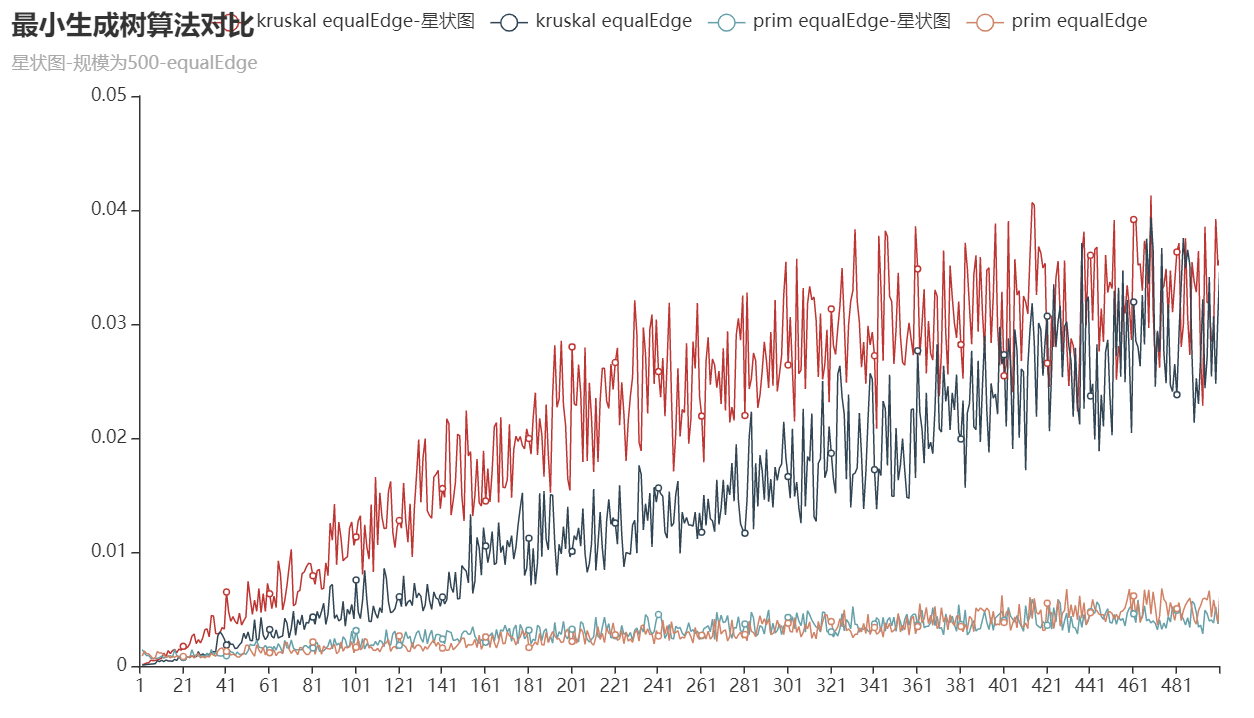
\includegraphics[width=0.95\textwidth]{assets/p500节点-等权-不同稀疏度.png}
        \end{minipage}
    }
    \subfigure[500节点排列权]{
        \begin{minipage}[t]{0.45\linewidth}
            \centering
            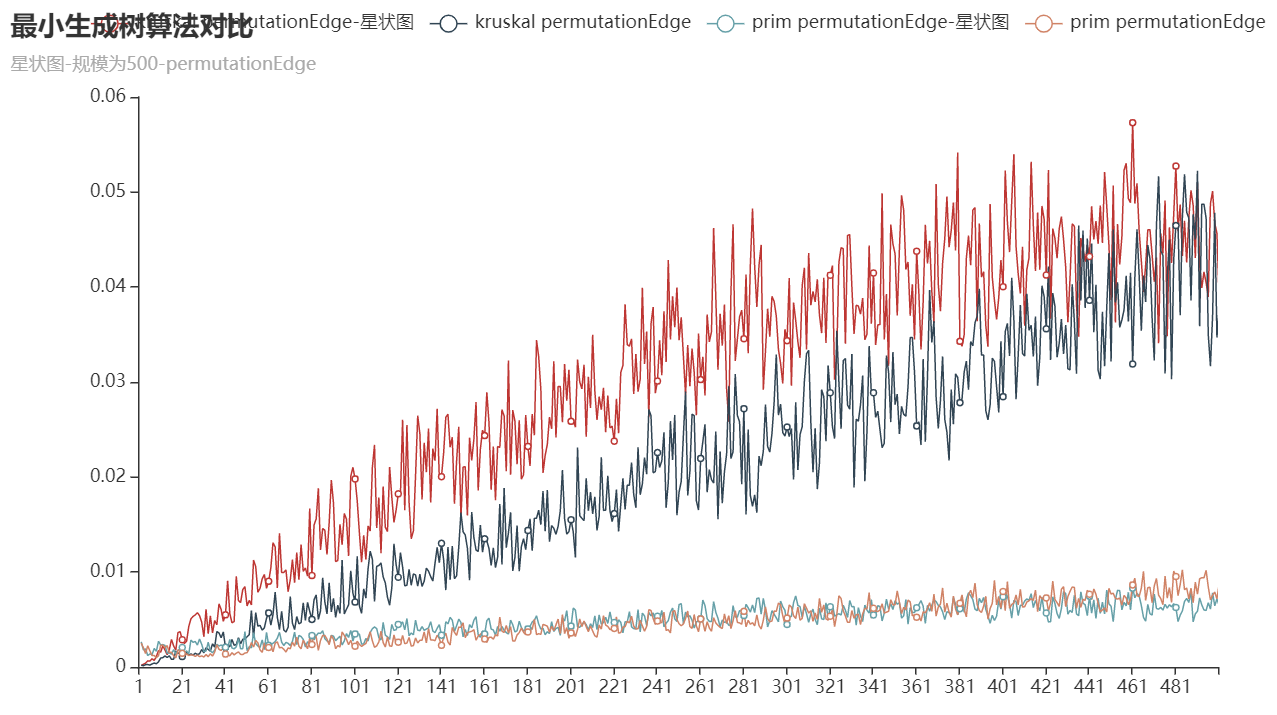
\includegraphics[width=0.95\textwidth]{assets/p500节点-排列权-不同稀疏度.png}
        \end{minipage}
    }
    
    \subfigure[500节点随机权]{
        \begin{minipage}[t]{0.45\linewidth}
            \centering
            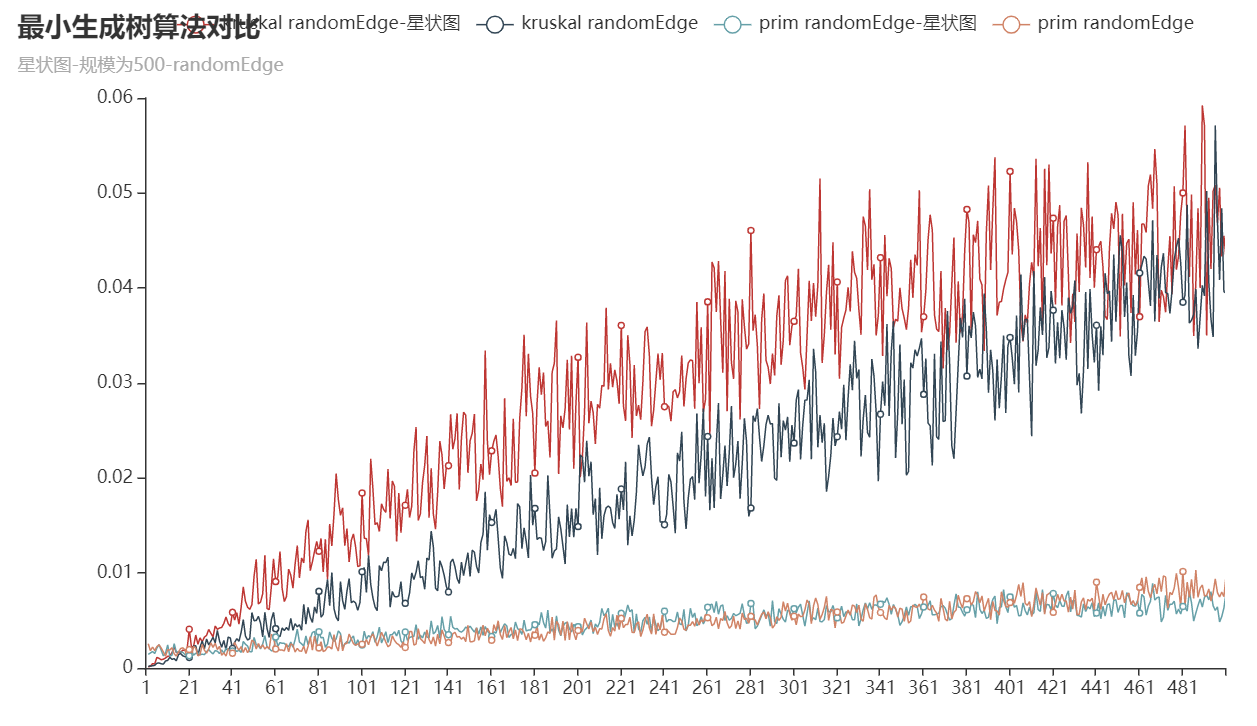
\includegraphics[width=0.95\textwidth]{assets/p500节点-随机权-不同稀疏度.png}
        \end{minipage}
    }
    \caption{不同加边方式的对比}
    \label{fig:pntest}
\end{figure}

比较看来,Prim算法表现因为受边数影响较小,所以在两组比较中表现出相对稳定的状态,但由于这种加边方式前期加边数较多,受边数影响较大的Kruskal就产生了明显的不同。

考虑到平均加边是每次加\(\frac{n-1}{2}\)条边,所以这样两种加边方式在初期的加边数有着较大差异,为了消除这种影响,实现控制变量,我们增大节点数,然后在加边的前200个情形中,我们近似认为添加边数相差2倍,并进行对齐操作,即将加边较多的星状图的情形的数据连续取样而加边较少的情形隔点取样,消除两个数据空间的分布密度的差异,相当于横轴拉伸2倍,从而获得的结果如图\ref{fig:pntest2000&5000}和\ref{fig:pntest10000},耗时就近似只和算法本身对于两种加边的不同适应性有关了。

\begin{figure}[htbp]
    \centering
    \subfigure[2000节点等权]{
        \begin{minipage}[t]{0.45\linewidth}
            \centering
            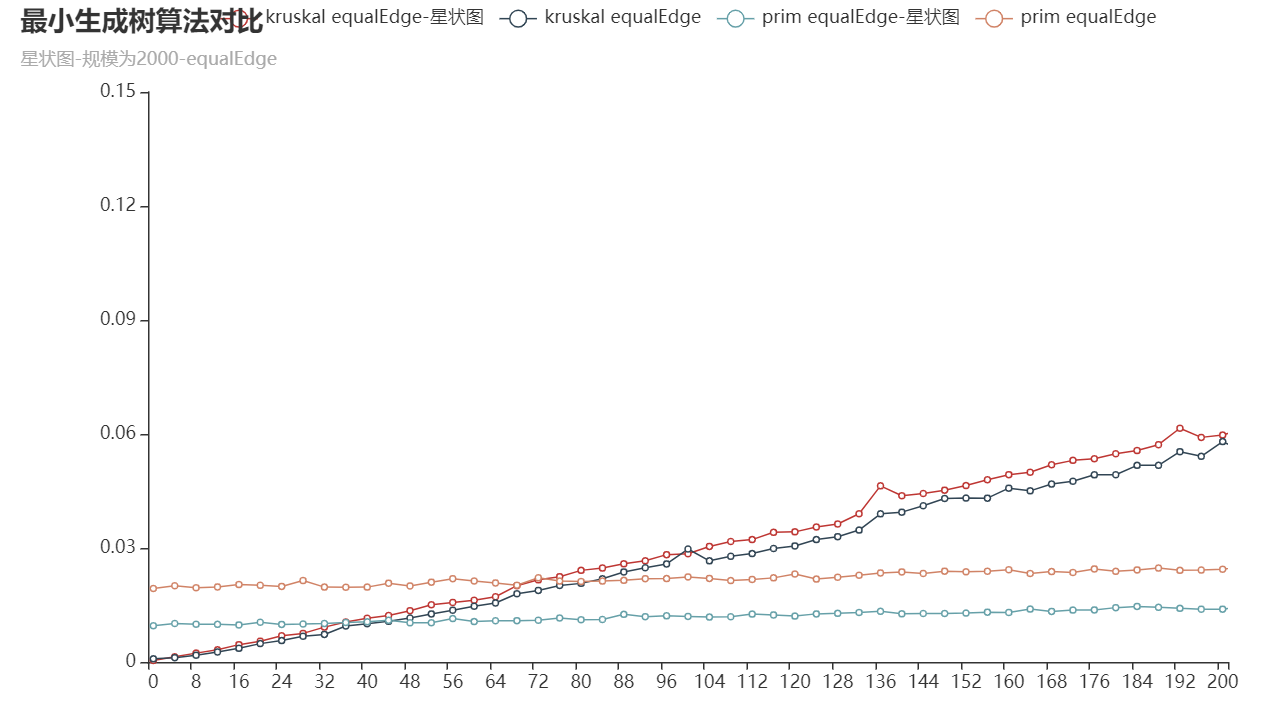
\includegraphics[width=0.95\textwidth]{assets/p2000节点-等权-不同稀疏度.png}
        \end{minipage}
    }
    \subfigure[2000节点排列权]{
        \begin{minipage}[t]{0.45\linewidth}
            \centering
            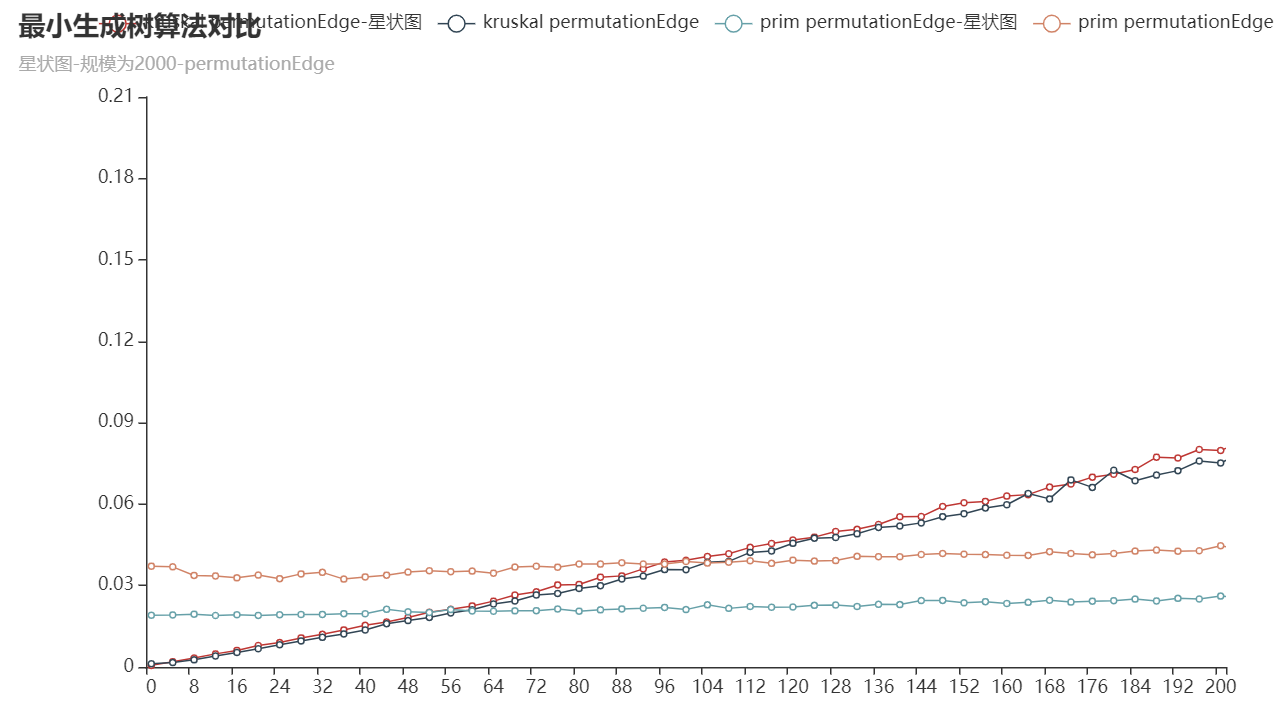
\includegraphics[width=0.95\textwidth]{assets/p2000节点-排列权-不同稀疏度.png}
        \end{minipage}
    }
    
    \subfigure[2000节点随机权]{
        \begin{minipage}[t]{0.45\linewidth}
            \centering
            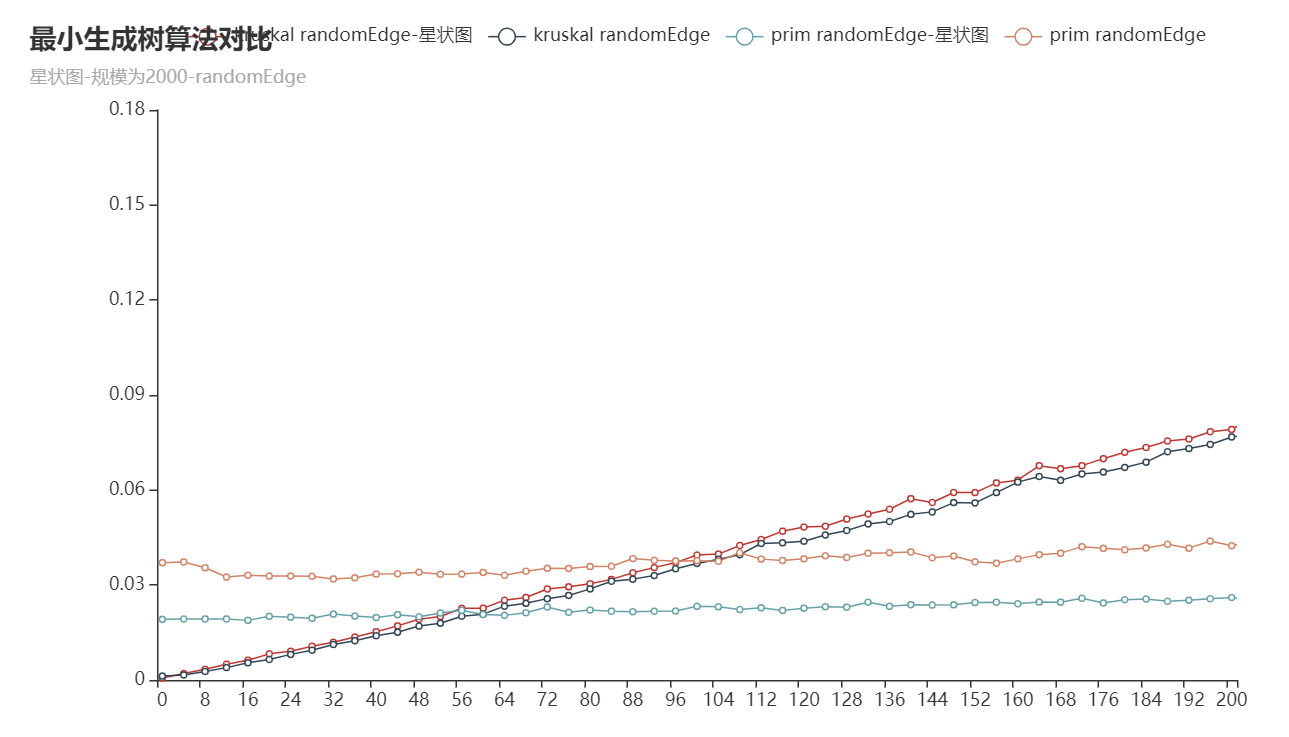
\includegraphics[width=0.95\textwidth]{assets/p2000节点-随机权-不同稀疏度.png}
        \end{minipage}
    }
    \subfigure[5000节点等权]{
        \begin{minipage}[t]{0.45\linewidth}
            \centering
            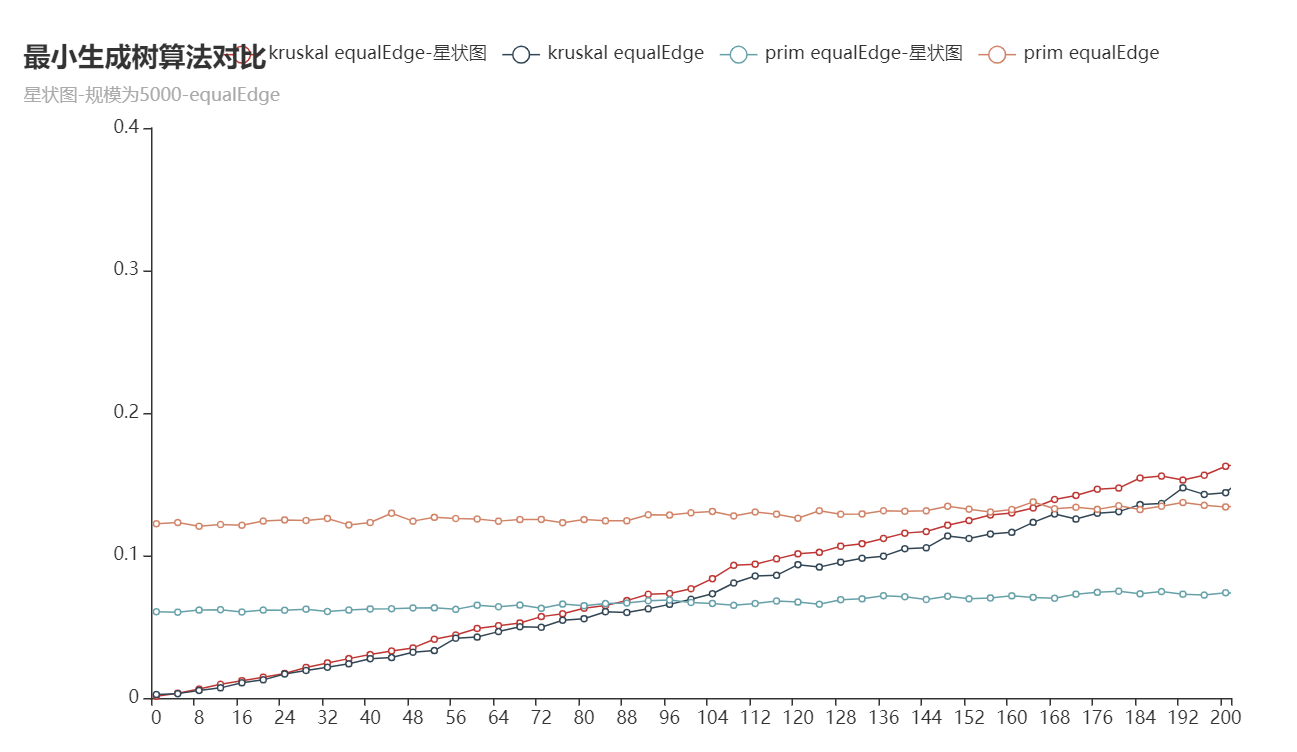
\includegraphics[width=0.95\textwidth]{assets/p5000节点-等权-不同稀疏度.png}
        \end{minipage}
    }

    \subfigure[5000节点排列权]{
        \begin{minipage}[t]{0.45\linewidth}
            \centering
            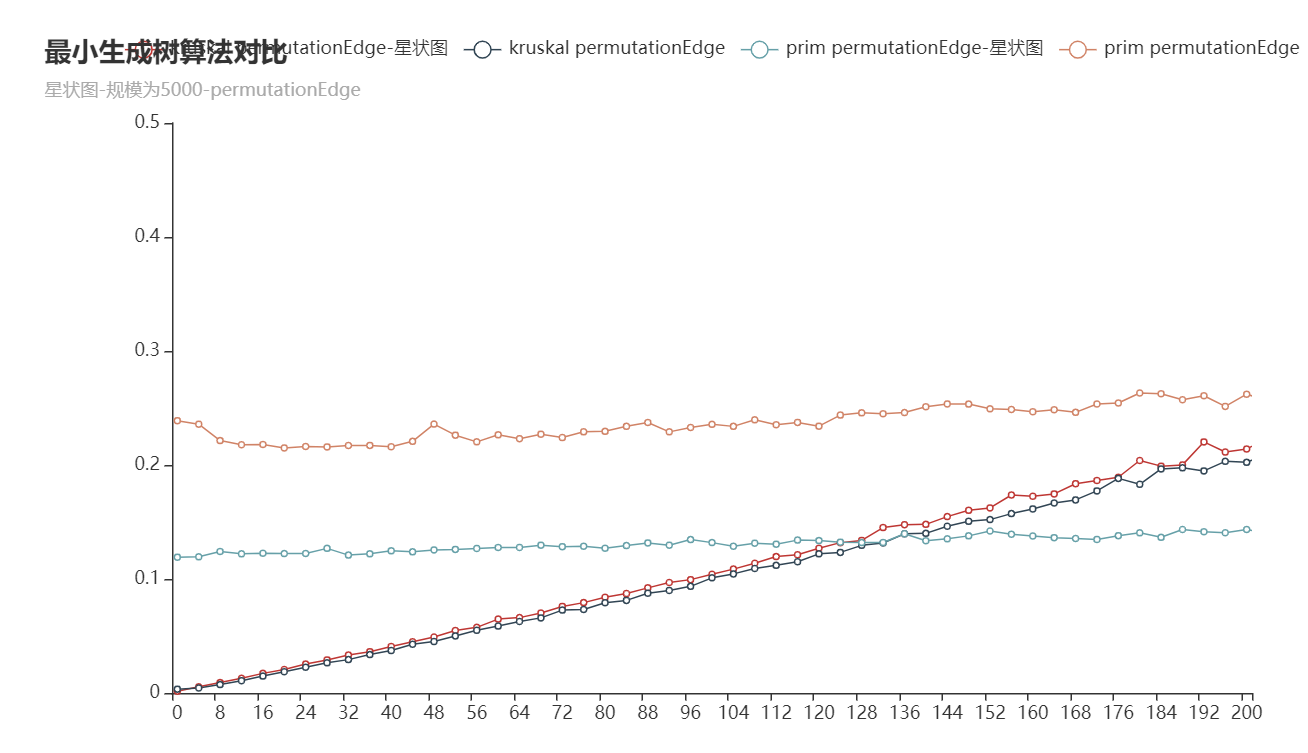
\includegraphics[width=0.95\textwidth]{assets/p5000节点-排列权-不同稀疏度.png}
        \end{minipage}
    }
    \subfigure[5000节点随机权]{
        \begin{minipage}[t]{0.45\linewidth}
            \centering
            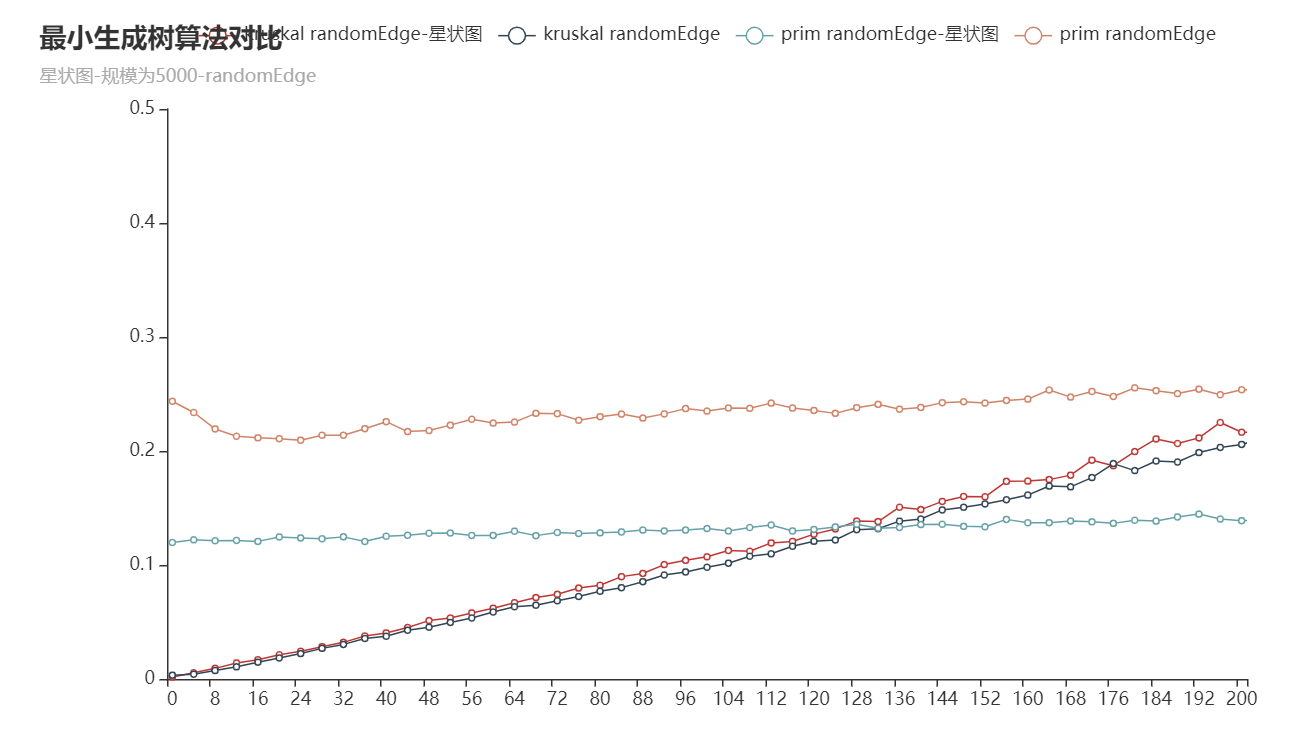
\includegraphics[width=0.95\textwidth]{assets/p5000节点-随机权-不同稀疏度.png}
        \end{minipage}
    }
    \caption{两种加边方式对齐之后的对比(1)}
    \label{fig:pntest2000&5000}
\end{figure}

\begin{figure}[htbp]
    \centering
    \subfigure[10000节点等权]{
        \begin{minipage}[t]{0.45\linewidth}
            \centering
            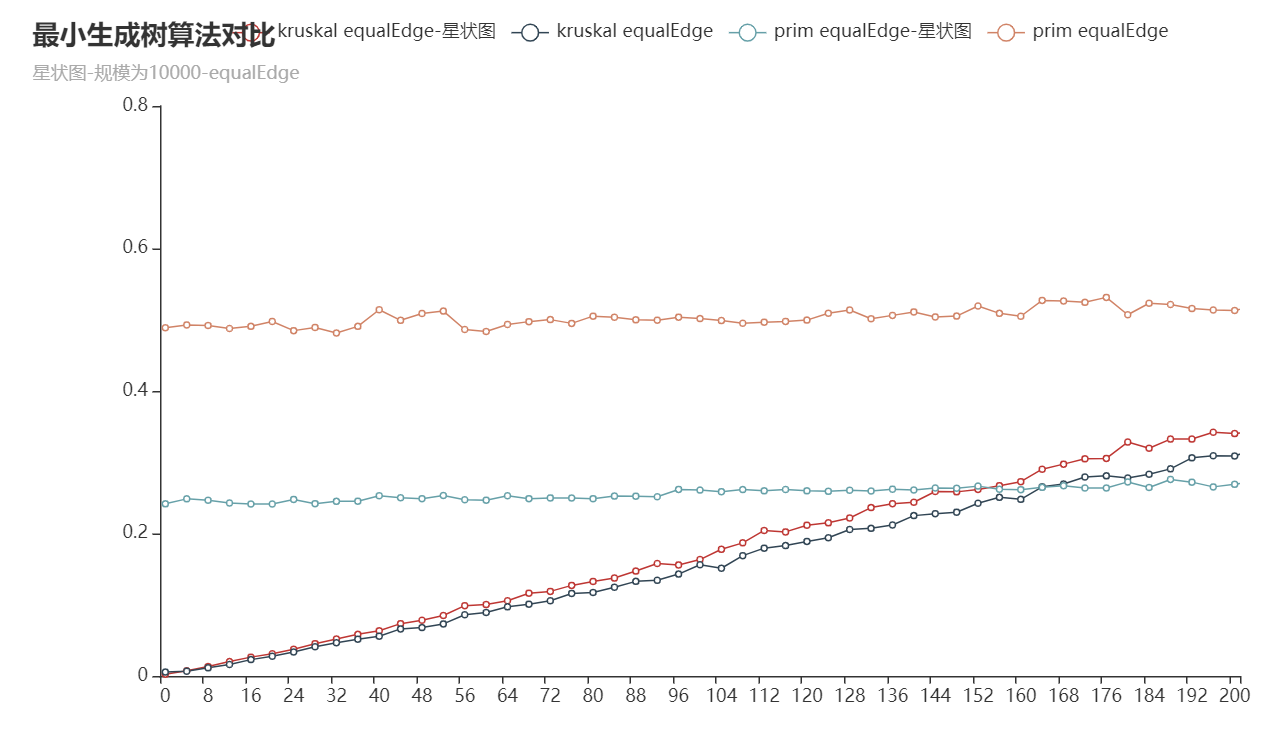
\includegraphics[width=0.95\textwidth]{assets/p10000节点-等权-不同稀疏度.png}
        \end{minipage}
    }
    \subfigure[10000节点排列权]{
        \begin{minipage}[t]{0.45\linewidth}
            \centering
            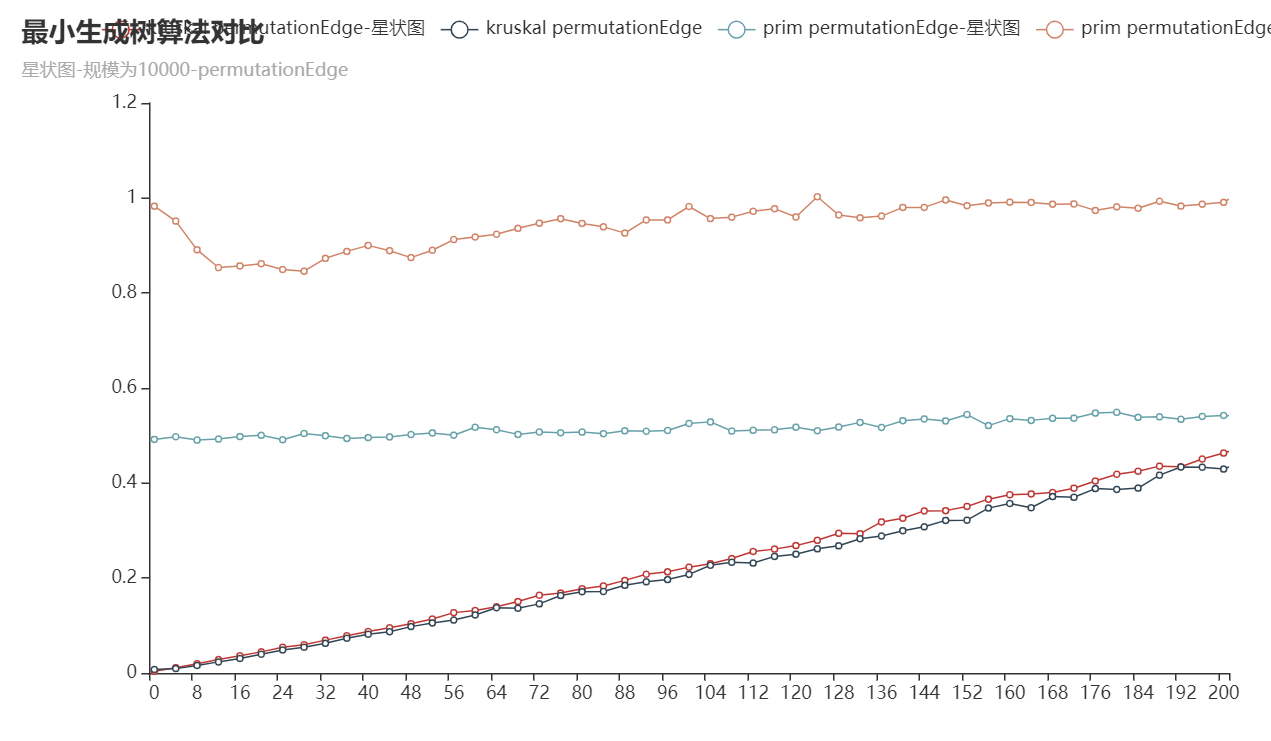
\includegraphics[width=0.95\textwidth]{assets/p10000节点-排列权-不同稀疏度.png}
        \end{minipage}
    }
    
    \subfigure[10000节点随机权]{
        \begin{minipage}[t]{0.45\linewidth}
            \centering
            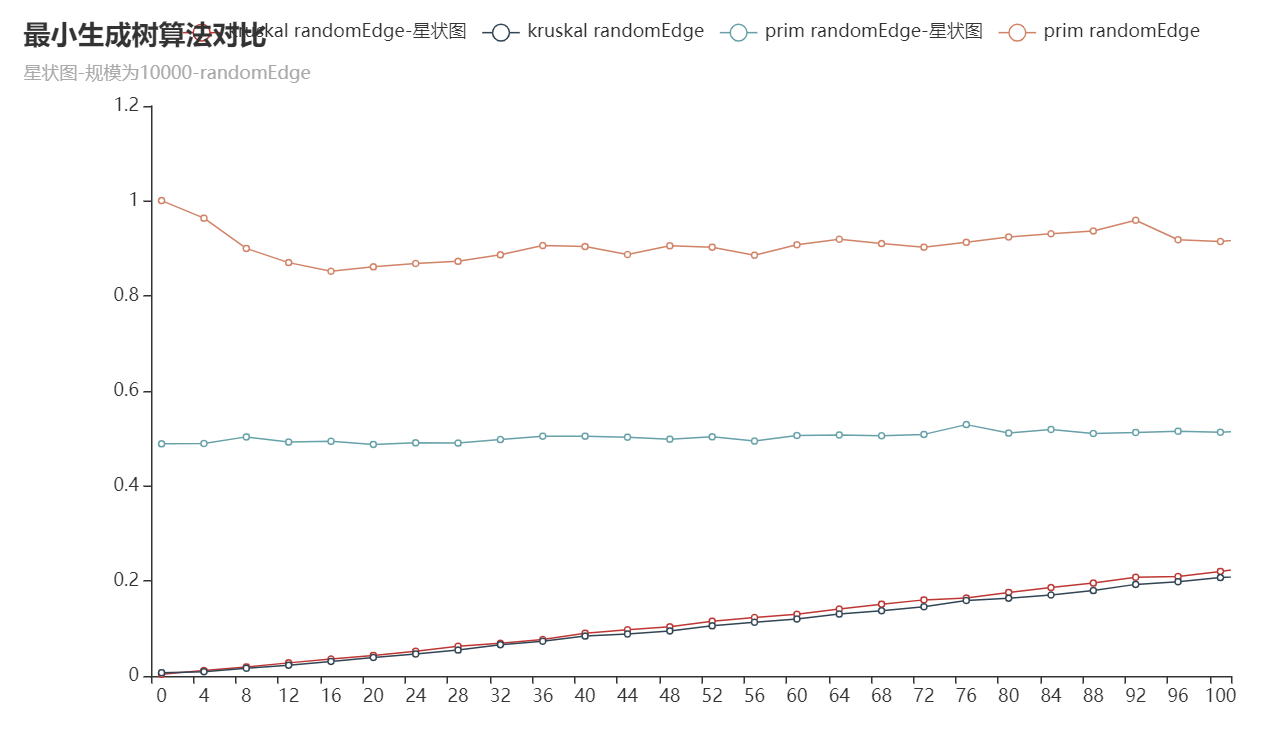
\includegraphics[width=0.95\textwidth]{assets/p10000节点-随机权-不同稀疏度.png}
        \end{minipage}
    }
    \caption{两种加边方式对齐之后的对比(2)}
    \label{fig:pntest10000}
\end{figure}

从图\ref{fig:pntest2000&5000}和\ref{fig:pntest10000}中可以看出,对两种算法的影响并不显著,这也是容易理解的,Kruskal的时间复杂度瓶颈在于排序。而Prim每个点处理完周边的边之后,其他点扩展仍然会遍历这些边,所以耗时增加并不明显。

\subsection{稀疏和稠密的极端情形}
算法分析课程中给出的“稠密用Prim”、“稀疏用Kruskal”已经经由上述实验完成了多维度验证,我们这里再给出树、完全图两种极稀疏和极稠密的图进行实验验证说明这个经验结论,如图\ref{fig:conclusion}。
\begin{figure}[htbp]
    \centering
    \subfigure[树]{
        \begin{minipage}[t]{0.45\linewidth}
            \centering
            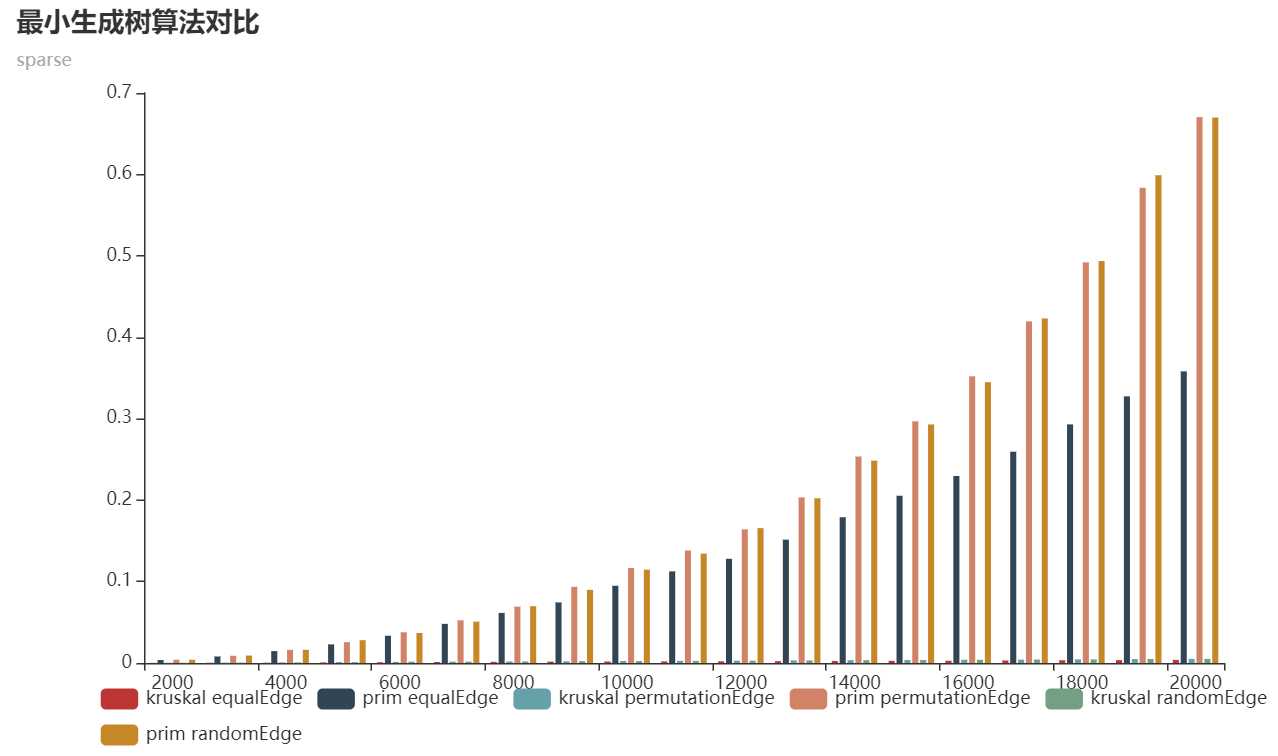
\includegraphics[width=0.95\textwidth]{assets/稀疏图-不同节点数.png}
        \end{minipage}
    }
    \subfigure[完全图]{
        \begin{minipage}[t]{0.45\linewidth}
            \centering
            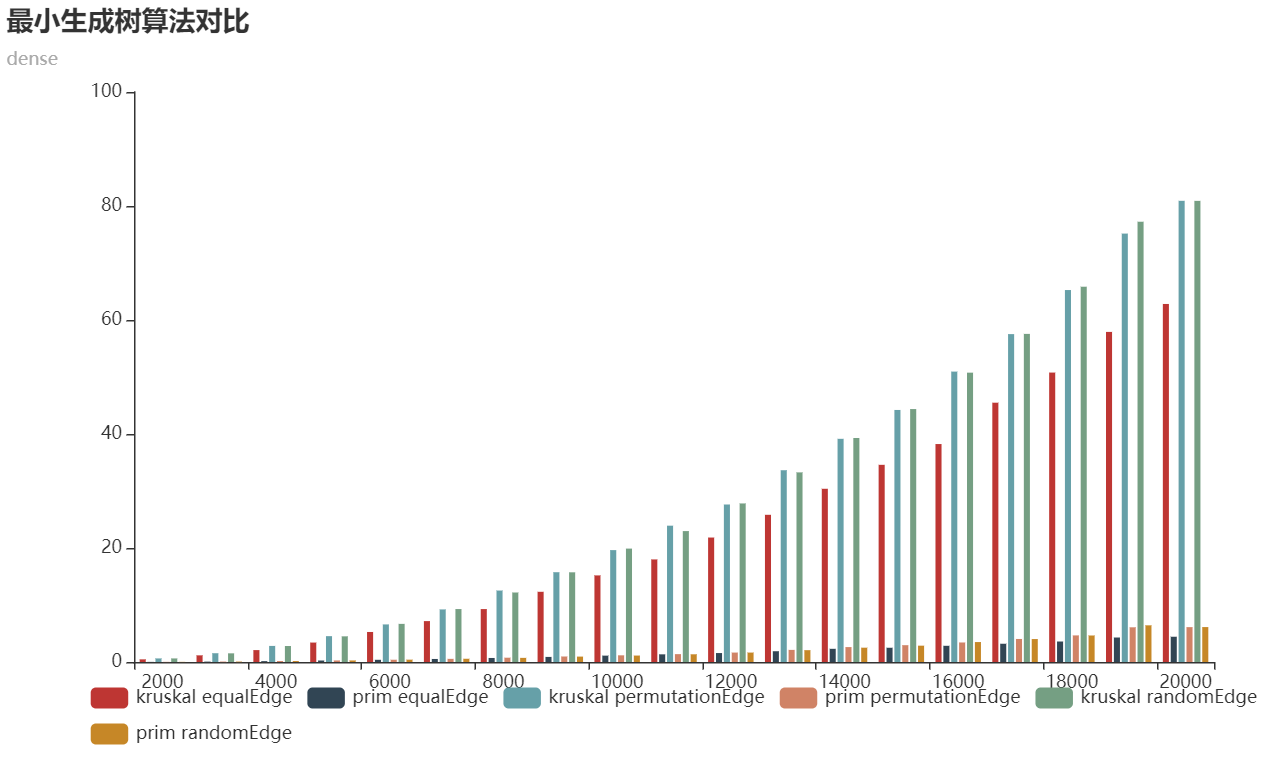
\includegraphics[width=0.95\textwidth]{assets/稠密图-不同节点数.png}
        \end{minipage}
    }
    \caption{稀疏适合适合Kruskal,稠密适合Prim}
    \label{fig:conclusion}
\end{figure}

\section{结论}
在实验中,我们对最小生成树的常用算法进行了对比。考虑到对比的有效性和结果的显著性,由于带有堆优化的Prim算法耗时极低,无可比性,所以我们重点对Kruskal算法和朴素Prim算法进行研究,实验中还采用三种分配权值的方式构建图。我们对节点数为100, 200, 500, 1000, 2000,5000,10000下不同疏密度的系列情况进行了实验。

另外除了平均赋边的方式,我们构建了星状图的特殊情况,进行了研究。对于这种从节点发散的图,Prim相比于Kruskal并无明显优势。

最终确定,对于Kruskal和朴素Prim算法来说,Kruskal仅在极稀疏的情况下优势明显,但在绝大多数较为稠密的图中,Prim算法都是更优的MST求解法。带有堆优化的Prim算法是更加优秀的MST算法。

\newpage
% \bibliographystyle{plain}
\bibliography{ref}

\end{document}

